
%% bare_conf.tex
%% V1.3
%% 2007/01/11
%% by Michael Shell
%% See:
%% http://www.michaelshell.org/
%% for current contact information.
%%
%% This is a skeleton file demonstrating the use of IEEEtran.cls
%% (requires IEEEtran.cls version 1.7 or later) with an IEEE conference paper.
%%
%% Support sites:
%% http://www.michaelshell.org/tex/ieeetran/
%% http://www.ctan.org/tex-archive/macros/latex/contrib/IEEEtran/
%% and
%% http://www.ieee.org/

%%*************************************************************************
%% Legal Notice:
%% This code is offered as-is without any warranty either expressed or
%% implied; without even the implied warranty of MERCHANTABILITY or
%% FITNESS FOR A PARTICULAR PURPOSE! 
%% User assumes all risk.
%% In no event shall IEEE or any contributor to this code be liable for
%% any damages or losses, including, but not limited to, incidental,
%% consequential, or any other damages, resulting from the use or misuse
%% of any information contained here.
%%
%% All comments are the opinions of their respective authors and are not
%% necessarily endorsed by the IEEE.
%%
%% This work is distributed under the LaTeX Project Public License (LPPL)
%% ( http://www.latex-project.org/ ) version 1.3, and may be freely used,
%% distributed and modified. A copy of the LPPL, version 1.3, is included
%% in the base LaTeX documentation of all distributions of LaTeX released
%% 2003/12/01 or later.
%% Retain all contribution notices and credits.
%% ** Modified files should be clearly indicated as such, including  **
%% ** renaming them and changing author support contact information. **
%%
%% File list of work: IEEEtran.cls, IEEEtran_HOWTO.pdf, bare_adv.tex,
%%                    bare_conf.tex, bare_jrnl.tex, bare_jrnl_compsoc.tex
%%*************************************************************************

% *** Authors should verify (and, if needed, correct) their LaTeX system  ***
% *** with the testflow diagnostic prior to trusting their LaTeX platform ***
% *** with production work. IEEE's font choices can trigger bugs that do  ***
% *** not appear when using other class files.                            ***
% The testflow support page is at:
% http://www.michaelshell.org/tex/testflow/



% Note that the a4paper option is mainly intended so that authors in
% countries using A4 can easily print to A4 and see how their papers will
% look in print - the typesetting of the document will not typically be
% affected with changes in paper size (but the bottom and side margins will).
% Use the testflow package mentioned above to verify correct handling of
% both paper sizes by the user's LaTeX system.
%
% Also note that the "draftcls" or "draftclsnofoot", not "draft", option
% should be used if it is desired that the figures are to be displayed in
% draft mode.
%
\documentclass[10pt, conference, compsocconf]{IEEEtran}
% Add the compsocconf option for Computer Society conferences.
%
% If IEEEtran.cls has not been installed into the LaTeX system files,
% manually specify the path to it like:
% \documentclass[conference]{../sty/IEEEtran}





% Some very useful LaTeX packages include:
% (uncomment the ones you want to load)


% *** MISC UTILITY PACKAGES ***
%
%\usepackage{ifpdf}
% Heiko Oberdiek's ifpdf.sty is very useful if you need conditional
% compilation based on whether the output is pdf or dvi.
% usage:
% \ifpdf
%   % pdf code
% \else
%   % dvi code
% \fi
% The latest version of ifpdf.sty can be obtained from:
% http://www.ctan.org/tex-archive/macros/latex/contrib/oberdiek/
% Also, note that IEEEtran.cls V1.7 and later provides a builtin
% \ifCLASSINFOpdf conditional that works the same way.
% When switching from latex to pdflatex and vice-versa, the compiler may
% have to be run twice to clear warning/error messages.






% *** CITATION PACKAGES ***
%
%\usepackage{cite}
% cite.sty was written by Donald Arseneau
% V1.6 and later of IEEEtran pre-defines the format of the cite.sty package
% \cite{} output to follow that of IEEE. Loading the cite package will
% result in citation numbers being automatically sorted and properly
% "compressed/ranged". e.g., [1], [9], [2], [7], [5], [6] without using
% cite.sty will become [1], [2], [5]--[7], [9] using cite.sty. cite.sty's
% \cite will automatically add leading space, if needed. Use cite.sty's
% noadjust option (cite.sty V3.8 and later) if you want to turn this off.
% cite.sty is already installed on most LaTeX systems. Be sure and use
% version 4.0 (2003-05-27) and later if using hyperref.sty. cite.sty does
% not currently provide for hyperlinked citations.
% The latest version can be obtained at:
% http://www.ctan.org/tex-archive/macros/latex/contrib/cite/
% The documentation is contained in the cite.sty file itself.






% *** GRAPHICS RELATED PACKAGES ***
%
\ifCLASSINFOpdf
  % \usepackage[pdftex]{graphicx}
  % declare the path(s) where your graphic files are
  % \graphicspath{{../pdf/}{../jpeg/}}
  % and their extensions so you won't have to specify these with
  % every instance of \includegraphics
  % \DeclareGraphicsExtensions{.pdf,.jpeg,.png}
\else
  % or other class option (dvipsone, dvipdf, if not using dvips). graphicx
  % will default to the driver specified in the system graphics.cfg if no
  % driver is specified.
  % \usepackage[dvips]{graphicx}
  % declare the path(s) where your graphic files are
  % \graphicspath{{../eps/}}
  % and their extensions so you won't have to specify these with
  % every instance of \includegraphics
  % \DeclareGraphicsExtensions{.eps}
\fi
% graphicx was written by David Carlisle and Sebastian Rahtz. It is
% required if you want graphics, photos, etc. graphicx.sty is already
% installed on most LaTeX systems. The latest version and documentation can
% be obtained at: 
% http://www.ctan.org/tex-archive/macros/latex/required/graphics/
% Another good source of documentation is "Using Imported Graphics in
% LaTeX2e" by Keith Reckdahl which can be found as epslatex.ps or
% epslatex.pdf at: http://www.ctan.org/tex-archive/info/
%
% latex, and pdflatex in dvi mode, support graphics in encapsulated
% postscript (.eps) format. pdflatex in pdf mode supports graphics
% in .pdf, .jpeg, .png and .mps (metapost) formats. Users should ensure
% that all non-photo figures use a vector format (.eps, .pdf, .mps) and
% not a bitmapped formats (.jpeg, .png). IEEE frowns on bitmapped formats
% which can result in "jaggedy"/blurry rendering of lines and letters as
% well as large increases in file sizes.
%
% You can find documentation about the pdfTeX application at:
% http://www.tug.org/applications/pdftex





% *** MATH PACKAGES ***
%
%\usepackage[cmex10]{amsmath}
% A popular package from the American Mathematical Society that provides
% many useful and powerful commands for dealing with mathematics. If using
% it, be sure to load this package with the cmex10 option to ensure that
% only type 1 fonts will utilized at all point sizes. Without this option,
% it is possible that some math symbols, particularly those within
% footnotes, will be rendered in bitmap form which will result in a
% document that can not be IEEE Xplore compliant!
%
% Also, note that the amsmath package sets \interdisplaylinepenalty to 10000
% thus preventing page breaks from occurring within multiline equations. Use:
%\interdisplaylinepenalty=2500
% after loading amsmath to restore such page breaks as IEEEtran.cls normally
% does. amsmath.sty is already installed on most LaTeX systems. The latest
% version and documentation can be obtained at:
% http://www.ctan.org/tex-archive/macros/latex/required/amslatex/math/





% *** SPECIALIZED LIST PACKAGES ***
%
%\usepackage{algorithmic}
% algorithmic.sty was written by Peter Williams and Rogerio Brito.
% This package provides an algorithmic environment fo describing algorithms.
% You can use the algorithmic environment in-text or within a figure
% environment to provide for a floating algorithm. Do NOT use the algorithm
% floating environment provided by algorithm.sty (by the same authors) or
% algorithm2e.sty (by Christophe Fiorio) as IEEE does not use dedicated
% algorithm float types and packages that provide these will not provide
% correct IEEE style captions. The latest version and documentation of
% algorithmic.sty can be obtained at:
% http://www.ctan.org/tex-archive/macros/latex/contrib/algorithms/
% There is also a support site at:
% http://algorithms.berlios.de/index.html
% Also of interest may be the (relatively newer and more customizable)
% algorithmicx.sty package by Szasz Janos:
% http://www.ctan.org/tex-archive/macros/latex/contrib/algorithmicx/




% *** ALIGNMENT PACKAGES ***
%
%\usepackage{array}
% Frank Mittelbach's and David Carlisle's array.sty patches and improves
% the standard LaTeX2e array and tabular environments to provide better
% appearance and additional user controls. As the default LaTeX2e table
% generation code is lacking to the point of almost being broken with
% respect to the quality of the end results, all users are strongly
% advised to use an enhanced (at the very least that provided by array.sty)
% set of table tools. array.sty is already installed on most systems. The
% latest version and documentation can be obtained at:
% http://www.ctan.org/tex-archive/macros/latex/required/tools/


%\usepackage{mdwmath}
%\usepackage{mdwtab}
% Also highly recommended is Mark Wooding's extremely powerful MDW tools,
% especially mdwmath.sty and mdwtab.sty which are used to format equations
% and tables, respectively. The MDWtools set is already installed on most
% LaTeX systems. The lastest version and documentation is available at:
% http://www.ctan.org/tex-archive/macros/latex/contrib/mdwtools/


% IEEEtran contains the IEEEeqnarray family of commands that can be used to
% generate multiline equations as well as matrices, tables, etc., of high
% quality.


%\usepackage{eqparbox}
% Also of notable interest is Scott Pakin's eqparbox package for creating
% (automatically sized) equal width boxes - aka "natural width parboxes".
% Available at:
% http://www.ctan.org/tex-archive/macros/latex/contrib/eqparbox/





% *** SUBFIGURE PACKAGES ***
%\usepackage[tight,footnotesize]{subfigure}
% subfigure.sty was written by Steven Douglas Cochran. This package makes it
% easy to put subfigures in your figures. e.g., "Figure 1a and 1b". For IEEE
% work, it is a good idea to load it with the tight package option to reduce
% the amount of white space around the subfigures. subfigure.sty is already
% installed on most LaTeX systems. The latest version and documentation can
% be obtained at:
% http://www.ctan.org/tex-archive/obsolete/macros/latex/contrib/subfigure/
% subfigure.sty has been superceeded by subfig.sty.



%\usepackage[caption=false]{caption}
%\usepackage[font=footnotesize]{subfig}
% subfig.sty, also written by Steven Douglas Cochran, is the modern
% replacement for subfigure.sty. However, subfig.sty requires and
% automatically loads Axel Sommerfeldt's caption.sty which will override
% IEEEtran.cls handling of captions and this will result in nonIEEE style
% figure/table captions. To prevent this problem, be sure and preload
% caption.sty with its "caption=false" package option. This is will preserve
% IEEEtran.cls handing of captions. Version 1.3 (2005/06/28) and later 
% (recommended due to many improvements over 1.2) of subfig.sty supports
% the caption=false option directly:
%\usepackage[caption=false,font=footnotesize]{subfig}
%
% The latest version and documentation can be obtained at:
% http://www.ctan.org/tex-archive/macros/latex/contrib/subfig/
% The latest version and documentation of caption.sty can be obtained at:
% http://www.ctan.org/tex-archive/macros/latex/contrib/caption/




% *** FLOAT PACKAGES ***
%
%\usepackage{fixltx2e}
% fixltx2e, the successor to the earlier fix2col.sty, was written by
% Frank Mittelbach and David Carlisle. This package corrects a few problems
% in the LaTeX2e kernel, the most notable of which is that in current
% LaTeX2e releases, the ordering of single and double column floats is not
% guaranteed to be preserved. Thus, an unpatched LaTeX2e can allow a
% single column figure to be placed prior to an earlier double column
% figure. The latest version and documentation can be found at:
% http://www.ctan.org/tex-archive/macros/latex/base/



%\usepackage{stfloats}
% stfloats.sty was written by Sigitas Tolusis. This package gives LaTeX2e
% the ability to do double column floats at the bottom of the page as well
% as the top. (e.g., "\begin{figure*}[!b]" is not normally possible in
% LaTeX2e). It also provides a command:
%\fnbelowfloat
% to enable the placement of footnotes below bottom floats (the standard
% LaTeX2e kernel puts them above bottom floats). This is an invasive package
% which rewrites many portions of the LaTeX2e float routines. It may not work
% with other packages that modify the LaTeX2e float routines. The latest
% version and documentation can be obtained at:
% http://www.ctan.org/tex-archive/macros/latex/contrib/sttools/
% Documentation is contained in the stfloats.sty comments as well as in the
% presfull.pdf file. Do not use the stfloats baselinefloat ability as IEEE
% does not allow \baselineskip to stretch. Authors submitting work to the
% IEEE should note that IEEE rarely uses double column equations and
% that authors should try to avoid such use. Do not be tempted to use the
% cuted.sty or midfloat.sty packages (also by Sigitas Tolusis) as IEEE does
% not format its papers in such ways.





% *** PDF, URL AND HYPERLINK PACKAGES ***
%
%\usepackage{url}
% url.sty was written by Donald Arseneau. It provides better support for
% handling and breaking URLs. url.sty is already installed on most LaTeX
% systems. The latest version can be obtained at:
% http://www.ctan.org/tex-archive/macros/latex/contrib/misc/
% Read the url.sty source comments for usage information. Basically,
% \url{my_url_here}.





% *** Do not adjust lengths that control margins, column widths, etc. ***
% *** Do not use packages that alter fonts (such as pslatex).         ***
% There should be no need to do such things with IEEEtran.cls V1.6 and later.
% (Unless specifically asked to do so by the journal or conference you plan
% to submit to, of course. )


% correct bad hyphenation here
\hyphenation{op-tical net-works semi-conduc-tor}


\usepackage{times}
\usepackage{CJKutf8}
\usepackage{mathrsfs}
\usepackage{textcomp}
\usepackage{verbatim}
\usepackage{amsmath}
\usepackage{amsfonts}
\usepackage{xspace}
\usepackage{xcolor}
\usepackage{url}
\usepackage{balance}
\usepackage{booktabs}
\usepackage{multirow}
\usepackage{rotating}
\usepackage{fancyvrb}
\usepackage{lastpage}
\usepackage{alltt}
\usepackage{etoolbox}
\usepackage{cleveref} % After hyperref, listings
\usepackage{fancyhdr}
\usepackage{listings}

\usepackage{caption}
\usepackage{subcaption}

\usepackage{tikz}
\usetikzlibrary{shapes,snakes}


\usepackage{amsmath}
\usepackage{amssymb}
\usepackage{wasysym}

%The given symbol or text (\text{mytext}) in a circle
%To be used always in math mode
\newcommand{\circlesign}[1]{ 
    \mathbin{
        \mathchoice
        {\buildcirclesign{\displaystyle}{#1}}
        {\buildcirclesign{\textstyle}{#1}}
        {\buildcirclesign{\scriptstyle}{#1}}
        {\buildcirclesign{\scriptscriptstyle}{#1}}
    } 
}


\newcommand\buildcirclesign[2]{%
    \begin{tikzpicture}[baseline=(X.base), inner sep=0, outer sep=0]
    \node[draw,circle] (X)  {\ensuremath{#1 #2}};
    \end{tikzpicture}%
}

\definecolor{lbcolor}{rgb}{0.9,0.9,0.9}
\lstset{
    tabsize=2,    
    language=C,
    basicstyle=\footnotesize\ttfamily,
    upquote=true,
    aboveskip={1.5\baselineskip},
    columns=fixed,
    extendedchars=false,
    showtabs=false,
    showspaces=false,
    showstringspaces=false,
    identifierstyle=\ttfamily,
    keywordstyle=\color[rgb]{0,0,1},
    commentstyle=\color[rgb]{0.026,0.112,0.095},
    stringstyle=\color[rgb]{0.627,0.126,0.941},
    numberstyle=\color[rgb]{0.205, 0.142, 0.73},
}


\usepackage{macro}
\newenvironment{CompactItemize}{\begin{itemize}}{\end{itemize}}
\def\code#1{{\texttt{#1}}}


\usepackage{colorhist}
 
\usepackage{minted}


\begin{document}
%
% paper title
% can use linebreaks \\ within to get better formatting as desired
\title{A Lightweight Log-based Deferred Update for Linux Kernel Scalability}


% author names and affiliations
% use a multiple column layout for up to two different
% affiliations

% \author{\IEEEauthorblockN{Authors Name/s per 1st Affiliation (Author)}
% \IEEEauthorblockA{line 1 (of Affiliation): dept. name of organization\\
% line 2: name of organization, acronyms acceptable\\
% line 3: City, Country\\
% line 4: Email: name@xyz.com}
% \and
% \IEEEauthorblockN{Authors Name/s per 2nd Affiliation (Author)}
% \IEEEauthorblockA{line 1 (of Affiliation): dept. name of organization\\
% line 2: name of organization, acronyms acceptable\\
% line 3: City, Country\\
% line 4: Email: name@xyz.com}
% }

% conference papers do not typically use \thanks and this command
% is locked out in conference mode. If really needed, such as for
% the acknowledgment of grants, issue a \IEEEoverridecommandlockouts
% after \documentclass

% for over three affiliations, or if they all won't fit within the width
% of the page, use this alternative format:
% 
%\author{\IEEEauthorblockN{Michael Shell\IEEEauthorrefmark{1},
%Homer Simpson\IEEEauthorrefmark{2},
%James Kirk\IEEEauthorrefmark{3}, 
%Montgomery Scott\IEEEauthorrefmark{3} and
%Eldon Tyrell\IEEEauthorrefmark{4}}
%\IEEEauthorblockA{\IEEEauthorrefmark{1}School of Electrical and Computer Engineering\\
%Georgia Institute of Technology,
%Atlanta, Georgia 30332--0250\\ Email: see http://www.michaelshell.org/contact.html}
%\IEEEauthorblockA{\IEEEauthorrefmark{2}Twentieth Century Fox, Springfield, USA\\
%Email: homer@thesimpsons.com}
%\IEEEauthorblockA{\IEEEauthorrefmark{3}Starfleet Academy, San Francisco, California 96678-2391\\
%Telephone: (800) 555--1212, Fax: (888) 555--1212}
%\IEEEauthorblockA{\IEEEauthorrefmark{4}Tyrell Inc., 123 Replicant Street, Los Angeles, California 90210--4321}}




% use for special paper notices
%\IEEEspecialpapernotice{(Invited Paper)}





% make the title area
\maketitle

%한글 버전으로 출력 하고 싶으면, korture를 Enable 해주시고, korefalse를 주석 처리 해주세요.
\newif\ifkor
\kortrue 
%\korfalse

\begin{abstract}
We propose a novel light weight concurrent updates method, \deferu, 
to improve performance scalability for Linux kernel on many-core systems
through eliminating lock contentions for update-heavy global data structures
during process spawning and optimizing update logs. 
The proposed \deferu is implemented into Linux kernel 4.5 and evaluated 
using representative benchmark programs. 
Our evaluation reveals that the Linux kernel with \deferu shows performance
improvement by ranging from Xx through Xx on a 120 core system.

We propose a novel light weight concurrent update method, \deferu, 
to improve performance scalability for Linux kernel on many-core systems
through eliminating lock contentions for update-heavy global data structures
during process spawning and optimizing update logs. 
The proposed \deferu is implemented into Linux kernel 4.5 and evaluated 
using representative benchmark programs. 
Our evaluation reveals that the Linux kernel with \deferu shows performance
improvement by ranging from Xx through Xx on a 120 core system.

We propose a novel light weight concurrent update method, \deferu, 
to improve performance scalability for Linux kernel on many-core systems
through eliminating lock contentions for update-heavy global data structures
during process spawning and optimizing update logs. 
The proposed \deferu is implemented into Linux kernel 4.5 and evaluated 
using representative benchmark programs. 
Our evaluation reveals that the Linux kernel with \deferu shows performance
improvement by ranging from Xx through Xx on a 120 core system.
\end{abstract}

\begin{IEEEkeywords}
component; formatting; style; styling;

\end{IEEEkeywords}


% For peer review papers, you can put extra information on the cover
% page as needed:
% \ifCLASSOPTIONpeerreview
% \begin{center} \bfseries EDICS Category: 3-BBND \end{center}
% \fi
%
% For peerreview papers, this IEEEtran command inserts a page break and
% creates the second title. It will be ignored for other modes.
\IEEEpeerreviewmaketitle



\ifkor
\begin{CJK}{UTF8}{}\CJKfamily{mj}
\fi
\section{Introduction} \label{sec:introduction}

%$$$$$$$$$$$$$$$$$$$$$$$$$$$$$$$$$$$$$$$$$$$$$$$$$$$$$$$$$$$$$$$$$$$$$$$$$$$$$$$$
%$$$$$$$$$$$$$$$$$$$$$$$$$$$$$$$$$$$$$$$$$$$$$$$$$$$$$$$$$$$$$$$$$$$$$$$$$$$$$$$$
%Background
%$$$$$$$$$$$$$$$$$$$$$$$$$$$$$$$$$$$$$$$$$$$$$$$$$$$$$$$$$$$$$$$$$$$$$$$$$$$$$$$$
\ifkor
최근 코어수가 증가하고 있다. 따라서 멀티코어에서 매니코어 시스템으로 바뀌고 있다. 
매니코어 시스템에 대한 운영체제 커널의 parallelism은 시스템 전체의 parallelism에서 가장 중요하다. 
만약 커널이 scale하지 않으면, 그 위에 동작하는 응용프로그램들도 역시 scale하지 않는다[].
이처럼 중요한 운영체제 커널 중 멀티코어 또는 매니코어 환경에서 많이 사용되는 운영체제가 리눅스 커널이다[].
하지만 리눅스 커널은 아직 확장성 문제가
있다~\cite{SilasBoydWickizer2010LinuxScales48}~\cite{Changwoo2016UMSF}.
확장성 문제 중 하나는 락 경합 때문에 발생하는 업데이트 직렬화
문제이다~\cite{Matveev2015RLU}~\cite{Dodds2015SCT}.
그 이유는 업데이트 오퍼레이션은 여러 쓰레드가 동시에 수행되지 못하기
때문이다~\cite{mckenney2011parallel}.
\else
%최근 number of core가 증가하고 있다. 따라서 multicore system에서 manycore system시스템으로 바뀌고
% 있다.
% Sentence #1:
With the increasing core counts, processors are changing from multi-core to
many-core systems.
%manycore system에 대한 operationg system kernel의 parallelism은 시스템 전체의
% parallelism에서 가장 중요하다.
% Sentence #1:
In many-core systems, parallelism of the operating system kernel has been an
important part for the whole the system parallelism.
%만약 kernel이 scale하지 않으면, 그 위에 동작하는 application들도 역시 scale하지 않는다[].
% Sentence #1:
If the kernel does not scale, applications depending on the shared
resources provided by the operating system kernel would not scale[].
%이처럼 중요한 operating system kernel 중 multicore or manycore 환경에서 많이
% 사용되는 operating system가 linux kernel이다[].
% Sentence #1:
Among operating systems, the scalable operating system is the Linux kernel
because the kernel community has made it scalable[].
%community has made it scalable.
%하지만 Linux kernel은 아직 scalability problem이
%있다~\cite{SilasBoydWickizer2010LinuxScales48}~\cite{Changwoo2016UMSF}.
% Sentence #1:
The Linux kernel, however, has some scalability
problems~\cite{SilasBoydWickizer2010LinuxScales48}~\cite{Changwoo2016UMSF}.
%scalability problem 중 하나는 lock contention 때문에 발생하는 update serialization 
%problem이다~\cite{Matveev2015RLU}~\cite{Dodds2015SCT}.
%그 이유는 update operation은 여러 thread 동시에 수행되지 못하기
%때문이다~\cite{mckenney2011parallel}.
% Sentence #1:
One of which is update serizlization due to its update lock
contention;update operations cannot run in
parallel~\cite{mckenney2011parallel}~\cite{Matveev2015RLU}~\cite{Dodds2015SCT}.
\fi


%$$$$$$$$$$$$$$$$$$$$$$$$$$$$$$$$$$$$$$$$$$$$$$$$$$$$$$$$$$$$$$$$$$$$$$$$$$$$$$$$
%$$$$$$$$$$$$$$$$$$$$$$$$$$$$$$$$$$$$$$$$$$$$$$$$$$$$$$$$$$$$$$$$$$$$$$$$$$$$$$$$
%Problem gernal
%$$$$$$$$$$$$$$$$$$$$$$$$$$$$$$$$$$$$$$$$$$$$$$$$$$$$$$$$$$$$$$$$$$$$$$$$$$$$$$$$
\ifkor
이처럼 업데이트 직렬화 문제를 해결하기 위해 여러 동시적 업데이트 방법 들이 연구되고
있다~\cite{Arbel2014ConcurrentRCU}~\cite{Matveev2015RLU}.
이러한 동시적 업데이트 방법들은 업데이트 비율에 따라 많은 성능 차이를
보인다.
이 중 높은 업데이트 비율을 가진 자료 구조 때문에 발생하는 학장성 문제를 해결하기 위한 여러 방법이 연구 되고
있다.
그 중 하나는 cache communication bottleneck을 줄인 log-based
알고리즘~\cite{Shalev2006PLS}~\cite{Hendler2010FC}~\cite{SilasBoydWickizerPth}을
사용하는 것이다.
Log-based 알고리즘은 업데이트가 발생하면, data structure의 업데이트 operation을
per-core 또는 atomic하게 log로 저장하고 read operation을 수행하기 전에 저장된 로그를 수행하는것이다 .
이것은 마치 CoW(Copy On Write)와 유사하다~\cite{PaulDetailLWN}.
\else
%update serialization 문제를 해결하기 위해 여러 concurrent updates
%방법 들이 연구되고 있다~\cite{Arbel2014ConcurrentRCU}~\cite{Matveev2015RLU}.
% Sentence #1:
In order to solve the update serialization problem, various concurrent update
methods have been proposed~\cite{Arbel2014ConcurrentRCU}~\cite{Matveev2015RLU}.
%이러한 concurrent updates 방법들은 update ratio에 따라 많은 성능 차이를
%보인다~\cite{Matveev2015RLU}.
% Sentence #1:
These methods show different performances depending on their update ratios.
%이 중 high update rate을 가진 data structure 때문에 발생하는 scalability problem를 해결하기 위한
% 여러 방법이 연구 되고 있다.
% Sentence #1:
In the case of a high update rates(update-heavy) data structure, the
update serialization problem can pose a scalability bottleneck.
%, so various methods have been studied.
%그 중 하나는 cache coherence traffic을 줄인 log-based
%알고리즘~\cite{Hendler2010FC}~\cite{SilasBoydWickizerPth}을
%사용하는 것이다.
% Sentence #1:
However, log-based algorithms~\cite{Hendler2010FC}~\cite{SilasBoydWickizerPth}
can solve this update serialization problem by reducing cache coherence-related
overheads for update-heavy data structures.
%Log-based 알고리즘은 update가 발생하면, data structure의 update operation을
%per-core 또는 atomic하게 log로 저장하고 read operation을 수행하기 전에 저장된 log를 수행하는것이다 .
% Sentence #1:
When update operations occur, Log-based algorithm logs the update
operation and applies all operation logs to the data structure
before read operation, so readers can read up to date data structure in a way
similar to CoW(Copy On Write)~\cite{PaulDetailLWN}.
%이것은 마치 CoW(Copy On Write)와 유사하다~\cite{PaulDetailLWN}.

\fi

%$$$$$$$$$$$$$$$$$$$$$$$$$$$$$$$$$$$$$$$$$$$$$$$$$$$$$$$$$$$$$$$$$$$$$$$$$$$$$$$$
%$$$$$$$$$$$$$$$$$$$$$$$$$$$$$$$$$$$$$$$$$$$$$$$$$$$$$$$$$$$$$$$$$$$$$$$$$$$$$$$$
%Problem 
%$$$$$$$$$$$$$$$$$$$$$$$$$$$$$$$$$$$$$$$$$$$$$$$$$$$$$$$$$$$$$$$$$$$$$$$$$$$$$$$$
\ifkor
S. Boyd-Wickizer et al.는 동기화된 타임스탬프 카운터(synchronized timestamp counters) 기반의
per-core log를 활용하여 update-heavy한 자료구조를 대상으로 동시적 업데이트 문제를
해결함과 동시에 cache communication bottleneck을 줄였다~\cite{SilasBoydWickizerPth}.
동기화된 타임스탬프 카운터 기반의 per-core log를 활용한 동시적 업데이트방법은
업데이트 부분만 고려했을 때, per-core에 데이터를 저장함으로 굉장히 높은 scalability를 가진다[].
하지만 per-core 기반의 동기화된 타임스탬프 카운터를 사용한 방법은 결국 timestamp merging and ordering 작업을
야기한다.
만약 코어 수가 늘어 날 경우, 로그를 자료 구조에 적용하는 과정에서 timestamp 때문에 발생하는 추가적인 sequential 프로세싱이
요구된다.
이것은 결국 확장성과 성능을 저해한다. 
\else
%S. Boyd-Wickizer et al. 는 synchronized timestamp counters 기반의 per-core log를
% 활용하여 update heavy한 data structure를 대상으로 concurrent updates 문제를
%해결함과 동시에 cache communication bottleneck을 줄였다~\cite{SilasBoydWickizerPth}.
% Sentence #1:
S. Boyd-Wickizer et al. proposed Oplog~\cite{SilasBoydWickizerPth}, where logs
update operations with synchronized timestamp counters solves concurrent
updates and cache communication bottleneck for its update-heavy data structure.
%Synchronized timestamp counters 기반의 per-core log를 활용한 concurrent updates 방법은
%update 부분만 고려했을 때, per-core에 데이터를 저장함으로 굉장히 높은 scalability를 가진다.
% Sentence #1:
The synchronized-timestamp-counters-based-method obtains outstanding
update-side scalability because it can record its operation logs without
cache communication overhead when it logs per-core memory.
%하지만 per-core 기반의 synchronized timestamp counters를 사용한 방법은 결국 timestamp
% merging and ordering 작업을 야기한다.
% Sentence #1:
However, the synchronized timestamp counters method may incur timestamp merging
and ordering process .
%만약 코어 수가 늘어 날 경우, resolving logs(merging, absorbing) may require
%additional sequential processing, which can limit scalalbility and
%performance.
% Sentence #1:
When core counts increase, resolving logs(merging, absorbing) may require
additional sequential processing, which can limit scalalbility and performance.
\fi



%$$$$$$$$$$$$$$$$$$$$$$$$$$$$$$$$$$$$$$$$$$$$$$$$$$$$$$$$$$$$$$$$$$$$$$$$$$$$$$$$
%$$$$$$$$$$$$$$$$$$$$$$$$$$$$$$$$$$$$$$$$$$$$$$$$$$$$$$$$$$$$$$$$$$$$$$$$$$$$$$$$
%Method
%$$$$$$$$$$$$$$$$$$$$$$$$$$$$$$$$$$$$$$$$$$$$$$$$$$$$$$$$$$$$$$$$$$$$$$$$$$$$$$$$
%
\ifkor
본 논문은 동기화된 타임스탬프 카운터를 이용함에 따라 생기는 추가적인 sequential processing 문제를
해결하기 위해 shared memory system을 위한 새로운 LDU(Lightweitgh log-based Deferred Update)를
개발하였다.
LDU는 타임스탬프 카운터가 필요한 operation log를 업데이트 순간 지우고, 매번 로그를 생성하지 않고 재활용하는 방법이다.
이로인해 synchronized timestamp counter 문제와 cache communication bottleneck 문제를 동시에
해결하였다.
해결 방법은 분산 시스템에서 사용하는 synchronized timestamp log기반의 concurrent updates 방식[]과
최소한의 shared-memory system의 hardware-based synchronization 기법(compare and swap,
test and set, atomic swap)을 조합하여 동시적 업데이트 문제를 해결하였다.
\else
%본 논문은 synchronized timestamp counters를 이용함에 따라 생기는 추가적인 sequencial processing 문제를
%해결하기 위해 shared memory system을 위한 새로운 LDU(Lightweitgh log-based Deferred
% Update)를 개발하였다.
% Sentence #1:
To solve the problem of sequential processing due to the synchronized timestamp
counters in shared memory system, we propose a novel lightweight log-based
deferred update method(LDU).
%LDU는 timestamp counters가 필요한 operation log를 update 순간 지우고, 매번 로그를 생성하지 않고 재활용하는
% 방법이다.
% Sentence #1:
LDU simply removes the operation log that requires timestamp counter at
update time and reuses the garbage log in the log's queue without creating new
log.
%이로인해 synchronized timestamp counter 문제와 cache communication bottleneck 문제를 동시에
%해결하였다.
% Sentence #1:
Therefore, we can eliminate the synchronized timestamp counter and the cache
communication bottleneck.
%해결 방법은 분산 시스템에서 사용하는 log기반의 concurrent updates 방식[]과
%최소한의 shared-memory system의 hardware-based synchronization 기법(compare and swap,
%test and set, atomic swap)을 조합하여 동시적 업데이트 문제를 해결하였다.
% Sentence #1:
We combine log-based concurrent update that is widely used in
the distributed system and the minimal hardware-based synchronization
method(compare and swap, test and set, atomic swap) that is used in shared-memory system.
\fi

\ifkor
이처럼 동기화된 타임스탬프 카운터를 제거함과 동시에, cache communication bottleneck 줄인
LDU는 기존 log-based 알고리즘들의 장점들을 모두 포함할 뿐만아니라 추가적인 장점을 가진다.
첫째로, update가 수행하는 시점 즉 로그를 저장하는 순간에는 fine-grain synchronization이 필요가 없다. 
따라서 synchronization 오버헤드 없이 concurrent updates를 수행할 수 있다
%둘째로, 저장된 update operation log를 coarse-grained lock과 함께 하나의 코어에서 수행하기 때문에,
%cache 효율성이 높아진다~\cite{Hendler2010FC}.
둘째로, 기존 여러 자료구조에 쉽게 적용할 수 있는 장점이 있다.
게다가 마지막으로, log를 저장하기 전에 로그를 삭제하므로 보다 빠르게 log의 수를 줄일 수 있다. 
\else
%이처럼 synchronized timestamp counters를 제거함과 동시에, cache communication bottleneck
% 줄인 LDU는 기존 log-based algorithm들의 장점들을 모두 포함할 뿐만아니라 추가적인 장점을 가진다.
% Sentence #1:
LDU has not only benefits of log-based algorithms but also additional benefits.
%첫째로, update가 수행하는 시점 즉 로그를 저장하는 순간에는 fine-grain synchronization이 필요가 없다. 
%따라서 lock에 대한 오버헤드 없이 concurrent updates를 수행할 수 있다
% Sentence #1:
First, log-based algorithms can remove synchronization overhead resulting in
reducing the cache invalidation traffic.
%둘째로 기존 여러 자료구조에 쉽게 적용할 수 있는 장점이 있다.
% Sentence #1:
Second, these techniques can be easily applied to other data structures.
%게다가 마지막으로, log를 저장하기 전에 로그가 삭제되므로 보다 빠르게 log의 수를 줄일 수 있다. 
% Sentence #1:
In addition, since LDU can eliminate the log before inserting the log's queue,
LDU's log management is efficient.
\fi

%$$$$$$$$$$$$$$$$$$$$$$$$$$$$$$$$$$$$$$$$$$$$$$$$$$$$$$$$$$$$$$$$$$$$$$$$$$$$$$$$
%$$$$$$$$$$$$$$$$$$$$$$$$$$$$$$$$$$$$$$$$$$$$$$$$$$$$$$$$$$$$$$$$$$$$$$$$$$$$$$$$
%Result
%$$$$$$$$$$$$$$$$$$$$$$$$$$$$$$$$$$$$$$$$$$$$$$$$$$$$$$$$$$$$$$$$$$$$$$$$$$$$$$$$

\ifkor
우리는 위와 같은 장점을 가지는 LDU를 리눅스 커널에서 high update rate 때문에 scalability 문제를 야기시키는
anonymous reverse mapping과 file reverse mapping에 적용하였다.
또한 우리는 LDU를 Linux 4.5.rc4에 구현하였고, fork-intensive 워크로드인
AIM7~\cite{AIM7Benchmark}, Exim~\cite{Exim} from MOSBENCH~\cite{MOSBENCH},
lmbench~\cite{mcvoy1996lmbench}를 대상으로 성능 개선을 보였다. 개선은 stock 리눅스 커널에 비해 120코어에서
각각 x,x,x 배이다.
\else
%우리는 위와 같은 장점을 가지는 LDU를 리눅스 커널의 fork scalability 문제를 야기시키는 2가지 reverse page
%mapping(anonymous pape mapping, file page mapping)에 적용하였다.
% Sentence #1:
To evaluate our approach, we applied LDU to Linux kernel reverse
page mappings(anonymous page mapping, file page mapping) that have the
problem of fork scalability bottleneck in Linux kernel because of
high update rates global data structure.
In addition, we implemented the LDU in a Linux 4.5.rc4.
We evaluated the performance and scalability using a fork-intensive workload-
AIM7~\cite{AIM7Benchmark}, Exim~\cite{Exim} from MOSBENCH~\cite{MOSBENCH},
lmbench~\cite{mcvoy1996lmbench}-our design improves throughput and execution
time on 120 core by 1.7x, 1.6x, 2.2x respectively, relative to stock Linux.
\fi


%$$$$$$$$$$$$$$$$$$$$$$$$$$$$$$$$$$$$$$$$$$$$$$$$$$$$$$$$$$$$$$$$$$$$$$$$$$$$$$$$
%$$$$$$$$$$$$$$$$$$$$$$$$$$$$$$$$$$$$$$$$$$$$$$$$$$$$$$$$$$$$$$$$$$$$$$$$$$$$$$$$
%Contribution 정리
%$$$$$$$$$$$$$$$$$$$$$$$$$$$$$$$$$$$$$$$$$$$$$$$$$$$$$$$$$$$$$$$$$$$$$$$$$$$$$$$$
\ifkor
\noindent
\textbf{Contributions.} Our research makes the following contributions:
\begin{itemize}
\item 우리는 high update rate를 가지는 data structure를 위한 새로운 log-based
concurrent updates 방법인 LDU를 개발하였다.
LDU는 동기화된 타임스탬프 카운터를 이용함에 따라 생기는 시간 정렬과 머징에 의한 추가적인 sequential processing 문제를
최소한의 hardware-based synchronization 기법을 사용하여 해결하였다.
LDU는 hardware-based synchronization 기법을 이용하여 LDU는 로그를 업데이트 순간 지우고 로그를 재활용한다.
\item 우리는 LDU을 practical한 many-core system인 intel xeon 120코어 위에 동작하는 리눅스 커널의
2가지 reverse mapping(anonymous, file)에 적용하여, fork scalability 문제를 해결하였다.
Fork 관련 벤치마크 성능은 워크로드 특성에 따라 1.6x부터 2.2x까지 개선되었다.
\end{itemize}
\else

\textbf{Contributions.} Our resesarch makes the following contributions:
\begin{itemize}
%\item 우리는 high update rate를 가지는 data structuer를 위한 새로운 log-based
%concurrnet updates 방법인 LDU를 개발하였다.
% Sentence #1:
%LDU는 동기화된 타임스탬프 카운터를 이용함에 따라 생기는 시간 정렬과 머징에 의한 추가적인 sequencial processing 문제를
%최소한의 hardware-based synchronization 기법을 사용하여 해결하였다.
%LDU는 hardware-based synchronization 기법을 이용하여 LDU는 로그를 업데이트 순간 지우고 로그를 재활용한다.
% Sentence #1:
\item We have developed a novel lightweight log-based deferred update method,
which can remove operation log that requires timestamp counter and reuses
the garbage log in log's queue;therefore, LDU can solve the Oplog's sequential processing problem due to the synchronized timestamp counters.
%\item 우리는 LDU을 practical한 manycore system인 intel xeon 120코어 위에 동작하는
% 리눅스 커널의 2가지 reverse mapping(anonymous, file)에 적용하여, fork scalability 문제를 해결하였다.
% Sentence #1:
\item 
We appiled LDU in Linux kernel to two reverse mapping(anonymous, file) on
practial 120core system to reduce fork scalability bottleneck.
%Fork 관련 벤치마크 성능은 워크로드 특성에 따라 1.6x부터 2.2x까지 개선되었다.
% Sentence #1:
Our design improved throughput and execution time on 120 core by 1.7x ~ 2.2x.
\end{itemize}

\fi


%$$$$$$$$$$$$$$$$$$$$$$$$$$$$$$$$$$$$$$$$$$$$$$$$$$$$$$$$$$$$$$$$$$$$$$$$$$$$$$$$
%$$$$$$$$$$$$$$$$$$$$$$$$$$$$$$$$$$$$$$$$$$$$$$$$$$$$$$$$$$$$$$$$$$$$$$$$$$$$$$$$
%Mapping
%$$$$$$$$$$$$$$$$$$$$$$$$$$$$$$$$$$$$$$$$$$$$$$$$$$$$$$$$$$$$$$$$$$$$$$$$$$$$$$$$
\ifkor
The rest of this paper is organized as follows.
Section 2 describes the background and the Linux scalability problem.
Section 3 describes the design of the LDU algorithm and 
Section 4 explains how to apply to Linux kernel.
section 5 explains our implementations in Linux and
Section 6 shows the results of the experimental evaluation. 
Finally, section 8 concludes the paper.
\else
The rest of this paper is organized as follows.
Section 2 describes the background and the Linux scalability problem.
Section 3 describes the design of the LDU algorithm and 
Section 4 explains how to apply the LDU to Linux kernel.
section 5 explains the implementations of LDU in Linux and
Section 6 shows the results of the experimental evaluation. 
Finally, section 7 concludes the paper.
\fi

%$$$$$$$$$$$$$$$$$$$$$$$$$$$$$$$$$$$$$$$$$$$$$$$$$$$$$$$$$$$$$$$$$$$$$$$$$$$$$$$$
%$$$$$$$$$$$$$$$$$$$$$$$$$$$$$$$$$$$$$$$$$$$$$$$$$$$$$$$$$$$$$$$$$$$$$$$$$$$$$$$$
% Reference Sentence 1
%$$$$$$$$$$$$$$$$$$$$$$$$$$$$$$$$$$$$$$$$$$$$$$$$$$$$$$$$$$$$$$$$$$$$$$$$$$$$$$$$
%
%





%$$$$$$$$$$$$$$$$$$$$$$$$$$$$$$$$$$$$$$$$$$$$$$$$$$$$$$$$$$$$$$$$$$$$$$$$$$$$$$$$
%Reference Sentence 2:LDU paper
%$$$$$$$$$$$$$$$$$$$$$$$$$$$$$$$$$$$$$$$$$$$$$$$$$$$$$$$$$$$$$$$$$$$$$$$$$$$$$$$$
% Ondemand로 로그를 지워 준다.
%Background
%With the drastic increase of CPU core counts in various high-end
%server systems, achieving performance scalability of operating systems
%running on such many-core systems has been an important issue in research
%communities.
%Linux has been naturally considered as a major target for the scalability
%improvement and a number of accomplishments are published.
%Early results include RCU~\cite{McKenney98} and hazard
%pointer~\cite{MagedMichael04a} to improve scalability for read-most data 
%structures in the Linux kernel. %for relatively low CPU core counts.
%Though the early results show certain level of improvement in scalability,
%it turned out that more significant portion of scalability limitation of
%Linux kernel is due to lock contention in update-heavy global data structures 
%including file reverse mappings and anonymous reverse mappings during
%spawning child processes~\cite{Andi2011adding}~\cite{Tim2013adding}. 
%Such update-heavy data structures cause serialization of the update operations
%leading to severe performance degradation. 

%Scaling operating systems to many-core architectures is one of the most
%important challenges in computing today. 
%One of the scalable operations system is Linux because the Linux kernel
%community has made it scalable.
%For example, read-mostly data structures in the Linux have been achieved
%considerable multi-core scaling by using RCU~\cite{McKenney98} and hazard
%pointer~\cite{MagedMichael04a}.
%However, the Linux kernel suffers from such scalability bottlenecks at high
%core counts.
%The Linux kernel on many-core processors can be
%bottlenecked by contended updates locks where processes share a global data
%structure.
%When a process spawns child process, reverse mapping using shared global
%data structure suffers from updates lock contention.
%Recent research shows how to run a fork in parallel with creating new reverse
%mapping data structure~\cite{SilasBoydWickizerPth}.
%More specifically, in order to perfect scalability of the fork, both the
%file reverse mapping and the anonymous reverse mapping can execute
%update concurrently without lock
%contention~\cite{Andi2011adding}~\cite{Tim2013adding}.

%The fundamental scalability problem of reverse mapping is their serialized
%update because operating systems are serialized at the update operation.

%To solve this problem, an existing approach is to make the update-heavy data
%structures as non-blocking~\cite{Harris2001Lockfree} based on
% \emph{compare-and-swap}(CAS).
%Introducing non-blocking data structures eliminates the update serialization
% problem during process spawning, but incurs additional issues due to
% inter-core communication
%bottlenecks and cache coherence system's write
% serialization~\cite{SilasBoydWickizerPth}.
%To overcome the issues caused by cache coherence system, S. Boyd-Wickizer et
% al. proposed Oplog~\cite{SilasBoydWickizerPth} where logs update operations
% with time stamps and actual updates are performed later when the updated data
% need to be read.
%While Oplog nicely solves the update serialization problem without any cache
% coherence-related overheads, the merging of the update logs recorded in
% multiple per-core data structures considering time stamps further causes
% performance overheads resulting in limited scalability
% improvement~\cite{McKenney2008ParallelProgramming}.

%Therefore, many researches have proposed non-blocking
%algorithms~\cite{Harris2001Lockfree} for concurrent data structure based on
%\emph{compare-and-swap}(CAS);nonetheless, this method may suffer from inter-core
%communication bottleneck, the cache coherence system serializes the
% writes~\cite{SilasBoydWickizerPth}.

%Another a existing solution is using the per-core processing like
%Oplog~\cite{SilasBoydWickizerPth}, which achieves scalability by logging in
%per-core memory.
%In fact, per-core approach may have best performance for the update-heavy data
%structure because of their partitioned data structures, whose updates can
%operate locally.
%The more-expensive reads, however, must merge across the entire per-core
%data;read operations are expensive~\cite{McKenney2008ParallelProgramming}.
%Therefore, their approach may be complex with regard to the read operation.
%This paper attacks this complexity as a result of the per-core processing.
%Even though they have generalized a per-core processing to the Oplog's library, 
%they use intricate optimizations, so their optimizations may be expensive with
%regard to the read operation.
%For example, they use the absorbing updates that removes the cancelable
%operation before the read.
%This operation may need to iterate previous operation log due to searching the
%cancelable operation log.
%Furthermore, reducing the memory use, they maintain per-core memory space.

%Method
%This paper proposes a novel concurrent update method, \deferu, applicable to
% Linux reverse mapping solving the problems 
%mentioned above: the overheads caused by inter-core communication bottlenecks
% and per-core log management with time stamps. 
%Our goal is to make the Linux fork scale to large numbers of cores using
%lightweight deferred processing algorithm.
%The fork scalability requires two challenges in designing a reverse mapping.
%First, this lightweight method should permit the concurrent updates not only to
%reduce the inter-core communication bottleneck but also to eliminate their 
%complexity.
%Second, this lightweight method should apply to Linux reverse mapping, and
%improve the Linux fork scalability.

%The \deferu is similar to Oplog in that it defers the actual update operations
% as late as possible to reduce serialization problems, but it uses a light
% weight global queue with non-blocking synchronization for update logs and
% eliminates time stamps required for per-core log management. 
%In addition, to optimize the log management and minimize the traversal
% overheads during reading, \deferu applies update-side absorbing algorithm based on atomic
%marking and thus efficiently find the operations to be canceled. 
%The evaluation of the proposed \deferu on Linux kernel 3.19.rc4 running on a
% 120 core system reveals that 
%the execution times could be improved by 1.7x, 1.6x, and 2.2x for 
%a fork-intensive workload-
%AIM7~\cite{AIM7Benchmark}, Exim from
%MOSBENCH~\cite{SilasBoydWickizer2010LinuxScales48}, and 
%lmbench~\cite{mcvoy1996lmbench}, respectively.

%Second, it uses a novel update-side absorbing that uses the atomic marking
%method, which allows \deferu to eliminate read-side traversal for finding the
%cancelable operation log;readers can improve performance.

%The proposed approach has the following advantages. 
%First, it can permits the reverse mapping to remove lock contention, so Linux's
%fork scalability has been improved.
%Second, using the lightweight update-side absorbing, \deferu can reduce
%complexity and improve readers performance.
%Finally, while per-core processing uses the time-stamp counter(e.g., RDTSCP,
%RDTSC) that depend on hardware, our method may not depend on hardware.

%We implemented the \deferu in a Linux 3.19.rc4 with modification of lock. 
%We evaluated the performance and scalability using a fork-intensive workload-
%AIM7~\cite{AIM7Benchmark}, Exim from
%MOSBENCH~\cite{SilasBoydWickizer2010LinuxScales48},
%lmbench~\cite{mcvoy1996lmbench}-our design improves throughput and execution
%time on 120 core by 1.7x, 1.6x, 2.2x respectively, relative to stock Linux.

%Mapping
%Paragraph 
%This paper is organized as follows. 
%Section 2 summarizes related works and compare our contributions to previous
%works. 
%Section 3 describes the design of the \deferu algorithm and 
%Section 4 explains how to apply to Linux kernel.
%section 5 explains our implementations in Linux and
%Section 6 shows the results of the experimental evaluation. 
%Finally, section 7 concludes the paper.
\section{Background and Problem}

%$$$$$$$$$$$$$$$$$$$$$$$$$$$$$$$$$$$$$$$$$$$$$$$$$$$$$$$$$$$$$$$$$$$$$$$$$$$$$$$$
% Paragraph 1: Linux Scalability : Fork intensive workload 문제점 설명 
%$$$$$$$$$$$$$$$$$$$$$$$$$$$$$$$$$$$$$$$$$$$$$$$$$$$$$$$$$$$$$$$$$$$$$$$$$$$$$$$$

\begin{figure}
  \begin{subfigure}[b]{0.25\textwidth}
    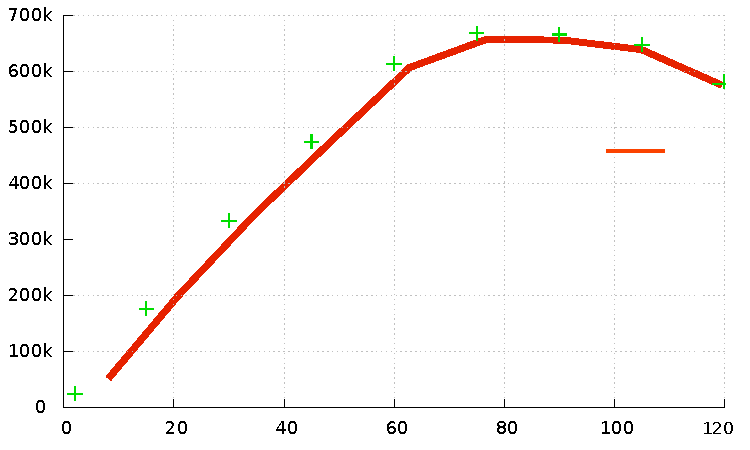
\includegraphics[width=\textwidth]{graph/aim7_default}
    \caption{aa}
  \end{subfigure}%
  \begin{subfigure}[b]{0.22\textwidth}
    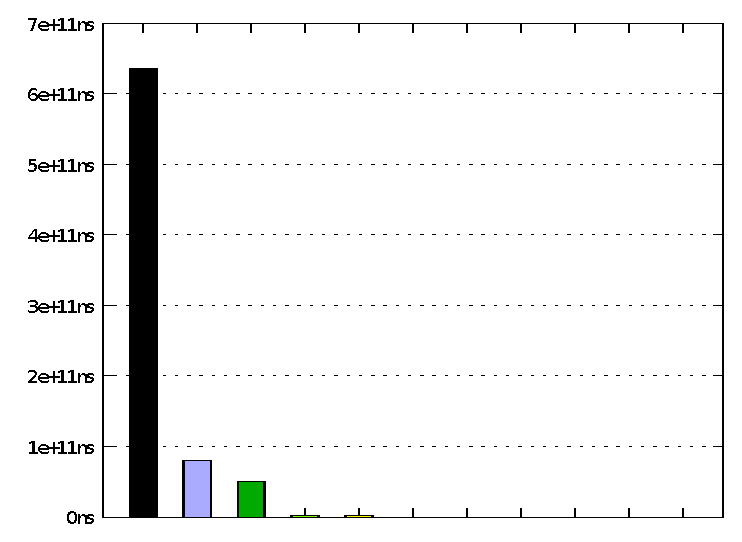
\includegraphics[width=\textwidth]{graph/lock_stat_anon}
    \caption{aa}
  \end{subfigure}
  \centering
  \caption{Scalability of AIM7 multiuser. This workload simultaneously create
  many processes.
  Up to 60 core, the stock Linux scale linearly, then they flattens out.}
  \label{fig:aim7_default}
\end{figure}
 
\ifkor

운영체제 커널의 paralleism은 시스템 전체의 parallesim에서 가장 중요하다. 
만약에 커널이 scale하지 않으면, 그 위에 동작하는 응용프로그램들도 역시 scale하지 않는다~\cite{Clements15SCR}.
우리는 이처럼 중요한 부분인 운영체제 커널중 multi-core에 최적화된 리눅스의 scalabiliy를 분석하기 위해, AIM7
multiuser[]를 가지고 scalability를 실험해보았다.
AIM7은 최근에도 scalability를 위해 reserach 진영과 리눅스 커널 진영에서도 활발히 사용되고 있는 벤치마크 중
하나이다~\cite{Bueso2015STP}~\cite{Bueso2014MCS}.
File system scalability를 최소화 하기 위해 temp filesystem~\cite{Rohland2001Tempfs}을
사용하였다.
This workload simultaneously create many processes.
Up to 60 core, the stock Linux scale linearly, then they flattens out.
\else


\fi

%$$$$$$$$$$$$$$$$$$$$$$$$$$$$$$$$$$$$$$$$$$$$$$$$$$$$$$$$$$$$$$$$$$$$$$$$$$$$$$$$
% Paragraph 2: Lockstat로 분석 결과 설명 
%$$$$$$$$$$$$$$$$$$$$$$$$$$$$$$$$$$$$$$$$$$$$$$$$$$$$$$$$$$$$$$$$$$$$$$$$$$$$$$$$

\ifkor
우리는 Scalability에 문제가 있는 120코어에서 리눅스의 Lockstat[]를 이용하여 락 경합을 분석하였다. 
먼저 멀티 프로세스 기반의 벤치마크인 AIM7을 동작시키고 동시에 120코어 대해서 락 경합을 분석하면 
그림 3과 같은 결과를 가진다. 
AIM7 벤치마크의 경우 상당히 많은 부분이 anonvma에서 쓰기 락 경합이 발생한다. 
이는 리눅스 역 매핑(reverse mapping)을 효율적으로 수행하기 위한 자료구인 anonvma를 
수많은 fork에 의해 프로세스를 생성하면서 발생하는 락 경합 문제이다. 
다음으로 우리는 anonvma의 lock 경합을 줄이기 위해, 임시로 fork에서 anonvma를 호출하는 부분과 read와
관련있는 pageswap이 안되도록 하고, 120코어를 대상으로 다시 Lock 경합을 분석하여 보았다.
이 때 부터 그동안 상대적으로 가려졌던 file reverse mapping에서 많은 락 경합이 발생되었다. 
이러한 anonvma reverse page mapping은 리눅스 커뮤니티에서 잘 알려진 락 경합
문제~\cite{Andi2011adding}~\cite{Tim2013adding}이고, file mapping에 대한 락 경합 문제는
Silas wikizer가 OpLog 논문을 통해 fork의 scalability 문제의 원인으로 제시한 부분이다.
본 연구의 분석 결과 둘 중 하나가 아니라 두 가지 락 모두 fork의 scalabililty 문제를 야기 시킨다.
즉 두가지 모두 개선해야지 fork의 scalalbility가 향상 된다. 
\else

\fi

%$$$$$$$$$$$$$$$$$$$$$$$$$$$$$$$$$$$$$$$$$$$$$$$$$$$$$$$$$$$$$$$$$$$$$$$$$$$$$$$$
% Paragraph 3: 리눅스 reverse page map의 write serialization 문제점
%$$$$$$$$$$$$$$$$$$$$$$$$$$$$$$$$$$$$$$$$$$$$$$$$$$$$$$$$$$$$$$$$$$$$$$$$$$$$$$$$

\ifkor
두가지 revserse page mapping의 근본적인 문제는 hight update operation에 대한 serialization 때문에
발생하는 문제이다.
이러한 revser page mapping은 page frame reclaiming을 위해 존재하며, 리눅스가 fork(), exit(),
and mmap() 시스템콜을 사용할 때 rmap을 update한다.
리눅스 커널은 reader들은 parallal 하게 동작할 수 있는 RW-lock 또는 RCU 같은 락 메카니즘이 있으나, 이러한 락은 결국
high update rate 앞에서는 serialization된다.
Update는 execulucive lock을 통해 보호해야하기 때문에, update rate 높은 상황이 발생하면 리눅스
커널은 결국 lock에 의해 serialized되어 scalability가 떨어진다.
\else

\fi

%$$$$$$$$$$$$$$$$$$$$$$$$$$$$$$$$$$$$$$$$$$$$$$$$$$$$$$$$$$$$$$$$$$$$$$$$$$$$$$$$
% Paragraph 4: update heavy한 상황에 대한 설명과 해결 방법에 대한 설명
%$$$$$$$$$$$$$$$$$$$$$$$$$$$$$$$$$$$$$$$$$$$$$$$$$$$$$$$$$$$$$$$$$$$$$$$$$$$$$$$$

\ifkor
이러한 high update rate이 발생하는 상황의 update serialization 문제에 대한 해결 방법들은 존재한다. 
근본적인 해결 방법은 update heavy한 상황이 발생하지 않도록 reverse page mapping 알고리즘을 새롭게 디자인하는 방법이
있다.
하지만 이미 오랜 시간 성능과 안정성이 검증된 알고리즘~cite{CorbetLWNRMAP}~\cite{CorbetLWNANON}을 새롭게
디자인 하는 일은 쉽지 않다.
보다 현실적인 방법은 concurrent updates를 위한, non-blocking data structure와
log-based 알고리즘을 사용하는 방법이 있다.
Non-blocking algorithms들은 hardware synchronized atomic 연산들을 활용하여 current 하게
update와 read를 수행하게 만든 data structure이다.
하지만 shared memory global value를 multipul CAS로 접근하여 bottlenecks이 생긴다.
due to inter-core communication overheads~\cite{SilasBoydWickizerPth}.
최근에는 Deu to the multipul CAS, inter-core communication overheads를 줄인 log-based
방법들이 연구되고 있다.
우리의 LDU도 이러한 log-based 기반 방법 활용하였으며, log-based 방법에 대한 설명은 다음 장에서 자세히 다룬다.
\else


\fi


%$$$$$$$$$$$$$$$$$$$$$$$$$$$$$$$$$$$$$$$$$$$$$$$$$$$$$$$$$$$$$$$$$$$$$$$$$$$$$$$$
%$$$$$$$$$$$$$$$$$$$$$$$$$$$$$$$$$$$$$$$$$$$$$$$$$$$$$$$$$$$$$$$$$$$$$$$$$$$$$$$$
%Reference Sentence 1
%$$$$$$$$$$$$$$$$$$$$$$$$$$$$$$$$$$$$$$$$$$$$$$$$$$$$$$$$$$$$$$$$$$$$$$$$$$$$$$$$






%$$$$$$$$$$$$$$$$$$$$$$$$$$$$$$$$$$$$$$$$$$$$$$$$$$$$$$$$$$$$$$$$$$$$$$$$$$$$$$$$
%Reference Sentence 2:LDU paper
%$$$$$$$$$$$$$$$$$$$$$$$$$$$$$$$$$$$$$$$$$$$$$$$$$$$$$$$$$$$$$$$$$$$$$$$$$$$$$$$$





\section{LDU Design}

%$$$$$$$$$$$$$$$$$$$$$$$$$$$$$$$$$$$$$$$$$$$$$$$$$$$$$$$$$$$$$$$$$$$$$$$$$$$$$$$$
%Paragraph 1: LDU의 특징을 간단한 설명과 이번장에 대한 설명(LDU의 특징을 요약하여 설명)
%$$$$$$$$$$$$$$$$$$$$$$$$$$$$$$$$$$$$$$$$$$$$$$$$$$$$$$$$$$$$$$$$$$$$$$$$$$$$$$$$

\ifkor
LDU는 리눅스 커널의 high update rates를 가진 data strcuture의 scalability를
해결하기 위한 log-based 방법 중에 하나이다.
동기화된 타임스탬프 카운터 기반의 per-core log를 활용한 동시적 업데이트방법은 결국 timestamp ordering and
merging 작업을 야기한다.
특히 코어 수가 늘어 날 경우, per-core 로그를 자료 구조에 적용하는 과정에서 추가적인 sequntial 프로세싱이 요구된다.
이것은 확장성과 성능을 저해한다. 
이러한 문제를 해결하기 위해, LDU는 log기반 방식의 concurrent updates 방법과 atomic synchronization
기능을 최소한으로 사용하도록 설계하였다.
따라서, LDU는 synchronized timestamp counter를 사용하는 방식의 timestamp를 제거함과 동시에 cache
communication overhead를 최소화 하였다.
예를 들어, high update rates data structure의 scalability 문제를 해결하기 위해, LDU는 update
operation 시점에 operation 로그를 atomic한 방법으로 삭제 또는 저장을 한다.
이를 위해 우리는 update-side abosrbing log, reuse garbage log라고 불리우는 2가지 최적화 방법을
사용하였다.
최적화 이후 남은 update operation에 대한 로그는 워크로드에 따라 global queue 또는 per-core queue에 저장할
수 있다.
본 장에서는 LDU의 Log-based 알고리즘과 어떻게 timestamp를 제거 했는지에 대한 디자인 측면에 대해서
설명한다.
\else
This section explains these algorithmic design aspects of LDU.
\fi



\subsection{Log-based Concurrent updates}

%$$$$$$$$$$$$$$$$$$$$$$$$$$$$$$$$$$$$$$$$$$$$$$$$$$$$$$$$$$$$$$$$$$$$$$$$$$$$$$$$
%Paragraph 1: Log 기반의 알고리즘 대략적인 설명 
%$$$$$$$$$$$$$$$$$$$$$$$$$$$$$$$$$$$$$$$$$$$$$$$$$$$$$$$$$$$$$$$$$$$$$$$$$$$$$$$$

\ifkor
Update heavy한 구조 때문에 발생하는 scalability 문제에 대한 해결책 중 하나는 Log-based 알고리즘을 사용하는 것이다.
Log-based 알고리즘은 lock을 피하기 위해 update가 발생하면, data structure의 update
operation(insert or remove)을 argument와 함께 저장하고, 주기적 또는 read operation을 수행하기 전에
applies the updates in all the logs to the data structure, so reader can read up to date data structure.
이러한 Log-based 방법은 마치 CoW(Copy on Write)와 유사하다.
즉, read 전에 저장된 log가 수행됨으로 read가 간혈적으로 수행되는 data structure에 적합한 방법이다.
\else

\fi


%$$$$$$$$$$$$$$$$$$$$$$$$$$$$$$$$$$$$$$$$$$$$$$$$$$$$$$$$$$$$$$$$$$$$$$$$$$$$$$$$
%Paragraph 2: Log 기반의 알고리즘의 장점
%$$$$$$$$$$$$$$$$$$$$$$$$$$$$$$$$$$$$$$$$$$$$$$$$$$$$$$$$$$$$$$$$$$$$$$$$$$$$$$$$
%
\ifkor
Update heavy한 구조를 위한 Log-based 방법은 총 4가지의 장점을 가진다. 
첫째로, update가 수행하는 시점 즉 로그를 저장하는 순간에는 lock이 필요가 없다. 
따라서 update를 concurrent하게 수행할 수 있을 뿐아니라, lock 자체가 가지고 있는 overall
coherence traffic is significantly reduced.
둘째로, 저장된 sequantial update operation log를 corse-grain lock과 함께 하나의 코어에서 수행하기
때문에, cache 효율성이 높아진다.
셋째로, 큰 수정 없이 기존 여러 데이터(tree, queue) structure에 쉽게 적용할 수 있는 장점이 있다.
마지막으로 저장된 log를 실제 수행하지 않고, 여러가지 optimization 방법을 사용하여 적은 operation으로 Log를 줄일 수
있다. 
LDU도 log-based approach를 따른다. 그러므로 앞에서 설명한 log-based 방법의 장점을 모두 가진다.
\else
Log-based approaches can help to support high update rates because
\fi



\subsection{Approach}

%$$$$$$$$$$$$$$$$$$$$$$$$$$$$$$$$$$$$$$$$$$$$$$$$$$$$$$$$$$$$$$$$$$$$$$$$$$$$$$$$
%Paragraph 1-삭제 예정: LDU는 another log-based 기법 : read before physical update 
%$$$$$$$$$$$$$$$$$$$$$$$$$$$$$$$$$$$$$$$$$$$$$$$$$$$$$$$$$$$$$$$$$$$$$$$$$$$$$$$$

\ifkor
%LDU는 먼저 lock 없이 concurrent Updates를 수행하기 위해, update를 수행하는 시점에서 lock이 필요없는 방법으로
%operation log를 저장 한다.
%따라서 lock이 없이 짐에 따라 scalability가 뿐만 아니라 lock 자체의 오버헤를 줄일 수 있다.
%저장된 Log는 불필요한 메모리 낭비를 줄이기 위해 주기적으로 flush하거나 또는 read 전에 호출되게 되는데, 이 때 LDU는 FC와
%같이 operation Log를 corse grain lock과 함께 single core에서 sequntial 프로세싱을 통해 수행한다. 
%따라서 cache의 miss를 줄여 성능을 향상시킨다[].
%다음으로 LDU는 Log-based 방법과 같이 기존 data structure를 많이 수정하지 않고도 다른 data structure에 쉽게
%적용할 수 있다.
\else
For update-heavy data structure LDU update before read operation;for example, it
similar to CoW(Copy On Write) method because acture update as long as possible
late.
\fi

%$$$$$$$$$$$$$$$$$$$$$$$$$$$$$$$$$$$$$$$$$$$$$$$$$$$$$$$$$$$$$$$$$$$$$$$$$$$$$$$$
%Paragraph 2: timestamp가 필요한 이유 : time-sensitive update operation log.
%$$$$$$$$$$$$$$$$$$$$$$$$$$$$$$$$$$$$$$$$$$$$$$$$$$$$$$$$$$$$$$$$$$$$$$$$$$$$$$$$
\ifkor
LDU는 update 순간 time-sensitive log를 제거함으로 synchronized timestamp counter 때문에 발생하는
문제를 해결하였다.
time-sensitive log란 순서가 바꿔서는 안되는 operation log이다. 
Synchronized timestamp가 근본적으로 필요한 이유는 when a process logs an insert
operation on one core, migrates to another core, and logs a remove operation, the remove should
eventually execute after the insert[]. 
본 논문에서는 이러한 time-sensitive log를 설명하기 위해, ~\cite{Clements15SCR}에서 사용한 심볼방법을
이용하였다.
먼저 $\oplus$와 $\ominus$는 각각 insert와 remove update operation을 의미한다.
바로 따라오는 심볼은 object의 명을 의미하고 색깔과 높낮이는 서로 다른 CPU를 의미한다.
\begin{center}
$\oplus$\inv{1}{A}, $\oplus$\inv{2}{B}, $\oplus$\inv{3}{C},$\oplus$\inv{1}{A},
$\oplus$\inv{3}{C}, $\oplus$\inv{1}{A}, $\oplus$\inv{2}{B},
$\oplus$\inv{3}{C},$\oplus$\inv{1}{A}, $\oplus$\inv{3}{C}
\end{center}
즉 위와 같이 수행되었을 경우 time-sensitive log인 $\oplus$\inv{1}{A}과 $\ominus$\inv{3}{C}에
대해서는 항상 timestamp에 맞게 수행되어야 한다.
여기서 중요한 사실은 time-sensitive operation log은 삭제해도 괜찮은 operation log들 이다.
여기서 insert-remove operation 또는 remove-insert operation을 가지는 
$\ominus$\inv{2}{B}, $\oplus$\inv{3}{C} 삭제되도 괜찮으며, 결국 남은 operation log은 같은
object에 대해서 insert 또는 remove operation만 남게 된다.
위의 log는 아래와 같이 non-time-sensitive한 operation만 남게 된다.
\begin{center}
$\oplus$\inv{3}{C}, $\oplus$\inv{1}{A}, $\oplus$\inv{2}{B},
$\oplus$\inv{3}{C}, $\oplus$\inv{1}{A}, $\oplus$\inv{2}{B}
\end{center}
LDU는 update-side absorbing 기술로 이러한 time-senstivive한 log를 update 순간 바로
지운다.
그 결과 synchronized timestamp의 필요성을 줄였다.
\else
If a process logs an insert operation on one core,
migrates to another core, and logs a remove operation, the remove should
eventually execute after the insert[OpLog].
\fi

%$$$$$$$$$$$$$$$$$$$$$$$$$$$$$$$$$$$$$$$$$$$$$$$$$$$$$$$$$$$$$$$$$$$$$$$$$$$$$$$$
%Paragraph 3:  time-sensitive update operation 삭제 방법: Update-side Abosrbing 
%$$$$$$$$$$$$$$$$$$$$$$$$$$$$$$$$$$$$$$$$$$$$$$$$$$$$$$$$$$$$$$$$$$$$$$$$$$$$$$$$

\ifkor
LDU는 time-senstivive한 log를 제거하기 위해 update-side absorbing이라는 방법을 사용한다.
이 방법은 만약 같은 object에 대해서 insert와 remove가 발생하였으면, 같은 object에
대해서, insert oepration과 remove operation에 대한 log를 update시점에 바로 바로 삭제하는 방법이다. 
이처럼 log가 삭제될 수 있는 이유는 operation log가 deferred로 수행하기 떄문에 가능하다. 
syncronized timestamp counters 기반의 OpLog도 이러한 log 삭제 방법 수행하여 최적화를 하였으나,
operation log가 서로 다른 코어에 존재하는 log 같은 경우에 log를 merge와 검색한 후 삭제를 해야한다. 
즉 syncronized timestamp counters 방법은 워크로드에 따라, 최적화를 위해 또 다른 sequntial 프로세싱이
요구된다.
하지만 LDU는 indivisual object를 대상으로 swap atomic operation을 사용하여
shared log 삭제하는 방법을 사용해서 이런 문제가 없다.

LDU의 update-side absorbing은 shared memory system의 swap operation을 사용한다.
이를 위해, LDU는 모든 object에 insert와 remove의 mark 필드를 추가해서 update-side
absorbing을 수행 하였다.
예를 들어 만약 A라는 object를 대상으로 insert-remove operation이 수행될 경우 처음 insert operation은
insert mark 필드에 표시하고 queue에 저장한다.
다음 remove operation 부터는 log를 queue에 저장하지 않고 insert에 표시한 mark 필드에 표시한 값만
atomic하게 지워주는 방식으로 진행된다.
다음으로 LDU는 log를 적용할 때, queue안에 log가 존재하더라도, mark 필드가 표시된 log만 실행한다.
이것은 swap이라는 상대적으로 가벼운 연산과 상대적으로 덜 share 하는 indivisaul global object의 mark filed를
사용해서 time-sensitive한 operation을 제거할 뿐만 아니라, 동시에 실제 operation을 수행하지 않고 log를 지워주는
효과를 가져주므로 성능이 향상된다. 

\else
\fi

%$$$$$$$$$$$$$$$$$$$$$$$$$$$$$$$$$$$$$$$$$$$$$$$$$$$$$$$$$$$$$$$$$$$$$$$$$$$$$$$$
%Paragraph 4: 리눅스의 update operation의 특징을 이용한 Update-side Abosrbing 
%$$$$$$$$$$$$$$$$$$$$$$$$$$$$$$$$$$$$$$$$$$$$$$$$$$$$$$$$$$$$$$$$$$$$$$$$$$$$$$$$

\ifkor
이처럼 update-side absorbing으로 log를 지울 수 있는 근본 이유는 리눅스 커널(freeBSD 커널 역시)
search가 two update operations(one to insert and one to remove an element)이 함수
외부해서 수행하는 구조이기 때문에 가능하다.
즉 리눅스의 data structure의 경우에는 search와 update가 분리되어 있어, 같은 update
operation이 연달아 호출되지 않는다.
LDU는 이러한 사실을 이용하여 update-side absorbing log를 개발 하였다. 
즉 리눅스의 data structure 구조는 search가 update operaton 외부에 있기 때문에 insert operation
다음에는 반드시 remove opration이 발생하고 remove operation 다음에는 반드시 insert operation이 발생하는
특징이 있다. %이러한 data structure는 search에서 이미 필터링이 되기 때문

이와 반대로 research 분야에서 많이 연구되는 CSDS(Concurrent search data
structures)~\cite{David2015ASYNCHRONIZED}의 방법들은 search가 update operation 내부에
존재하는 구조로 되어 있다.
따라서 같은 key값의 노드에 대해서 insert-insert 또는 remove-remove 순서로 동작할 수 있다.
이처럼 CSDS 알고리즘일 경우에는 LDU를 적용하지 못하는 limitation이 있다.
하지만 본 연구는 리눅스 커널과 같은 practical한 data structure에 초점을 맞추었기 때문에, 
research 분야에 많이 연구되고 있는 CSDS 알고리즘은 고려하지 않았다.
아직 CSDS의 non-blocking 알고리즘들은 garbage collector~\cite{AlBahra2013NAS},
iteration~\cite{petrank2013lock}, ordering~\cite{zhang2013practical}여러
practical한 이유로 C언어로 구현된 리눅스 커널 등에 적용하기에는 아직 한계가 있다.
\else
\fi

%$$$$$$$$$$$$$$$$$$$$$$$$$$$$$$$$$$$$$$$$$$$$$$$$$$$$$$$$$$$$$$$$$$$$$$$$$$$$$$$$
%Paragraph 5: 최적화 방법 reusing garbage object : 
%$$$$$$$$$$$$$$$$$$$$$$$$$$$$$$$$$$$$$$$$$$$$$$$$$$$$$$$$$$$$$$$$$$$$$$$$$$$$$$$$

\ifkor
LDU의 또 다른 최적화 기법은 update-side absorbing 때문에 취소된 garbage log를 재활용하는 것이다.
이 garbage log는 queue에는 존재하지만 update-side aborsrbing 때문에 취소 되어 garbage가 되어 queue에
보관되어 있는 log이다. 
이러한 garbage log일 경우 다음 update operation에 대해서는 해당 로그를 새로 많들어 넣지 않고 기존 로그를 재활용하는
방법이다.
예를 들어 A라는 오브젝트에 대해서 insert-remove-insert 순서로 update가 수행될 경우, 세번째 insert 명령어는
queue에 들어가 있지만 update-side absorbing 때문에 최소되어 insert mark filed가 zero인
경우(garbage object)이다.
이러한 경우, 다음 insert operation에 대해서는 새로운 log를 list에 연산으로 다시 넣지 않고, 해당 object의 mark
필드만 변경하여 log를 재활용하는 방법을 사용한다.
\else
\fi


%$$$$$$$$$$$$$$$$$$$$$$$$$$$$$$$$$$$$$$$$$$$$$$$$$$$$$$$$$$$$$$$$$$$$$$$$$$$$$$$$
%Paragraph 6: log를 저장하는 queue는 non-blocking queue를 사용
%$$$$$$$$$$$$$$$$$$$$$$$$$$$$$$$$$$$$$$$$$$$$$$$$$$$$$$$$$$$$$$$$$$$$$$$$$$$$$$$$
\ifkor
LDU는 queue의 위치(global or per-core)에 대한 의존성을 없애기 위해 log를 항상 non-blocking queue에
저장한다.
따라서 log를 저장하는 시점에 대해서 global lock 또는 per-core lock을 제거 하였다.
LDU는 head 포인터에 대한 CAS 연산을 최대한 줄인 multiple producers and single
consumer에 기반하는 non-blocking queue를 이용하였다.
이러한 큐는 이미 Linux 커널에 Lock-less list~\cite{HuangLocklessList}라는 이름으로 구현되어 있으며, 이미
커널에 많은 부분에 사용되고 있다.
이 큐는 다른 non-blocking list[][][]와 다르게, insert operation을 항상 처음 노드에 삽입함에
따라, CAS가 발생되는 횟수를 상대적으로 줄일 수 있다.
게다가 single consumer를 고려 했기 때문에, remove를 위한 복잡한 알고리즘이 필요없다. 
예를 들어 single consumer는 operation log 전체를 얻기 위해, xchg 명령을 사용하여 head pointer를
NULL로 atomic하게 제거한다. 
결론적으로 LDU는 queue의 위치에 따른 의존성을 제거하고, head pointer의
CAS fail 때문에 발생하는 multiple CAS를 최소화 하기 위해, Linux 커널에 있는 Lock-less list를 활용 하였다.
\else
\fi


%$$$$$$$$$$$$$$$$$$$$$$$$$$$$$$$$$$$$$$$$$$$$$$$$$$$$$$$$$$$$$$$$$$$$$$$$$$$$$$$$
%Paragraph 7: 두 종류의 queue를 지원하는 이유 : log를 저장하도록 설계 이유는 서로 장 단점이 있음 : (option)
%$$$$$$$$$$$$$$$$$$$$$$$$$$$$$$$$$$$$$$$$$$$$$$$$$$$$$$$$$$$$$$$$$$$$$$$$$$$$$$$$

\ifkor
LDU는 log를 저장하기 위해, global 또는 per-core queue 모두 이용할 수 있게 설계하였다.
즉 저장하는 방법이 global queue이면 global non-blocking queue를 이용하고, per-core queue이면
per-core 메모리에 non-blocking queue를 저장하여 사용하였다. 
이러한 두가지 queue를 지원하도록 한것은 서로 장단점을 가지고 있기 때문이다.
예를 들어 일반적으로 per-core 방법이 굉장히 높은 scalability를 가진다고 하지만, 본 연구 결과 data
structure의 head를 가지는 root object가 굉장히 많이 생성되는 워크로드일 경우,
per-core 방법은 너무 많은 메모리를 요구한다.
만약 적은 메모리를 사용할 경우 오히려 성능이 떨어지는 결과를 가진다[section x].
즉 log-based 방법은 워크로드에 맞는 queue를 사용해야한다. 

이와 같이 LDU의 두가지 queue는 서로 장단점을 가지고 있다. 
먼저 global queue의 장점은 광장히 simple하여 어떻한 data structure간에 쉽게 적용이 가능하다.
global queue를 사용한 방법은 LDU의 light-weight한 queue사용과 update-side absorbing log와
reuse garbage log 기법등으로 global head 포인터에 대한 CAS operation 사용을 줄였지만, 여전히 global
header에 CAS가 사용되고 있다. 
따라서 cache coherence traffic issue가 여전히 남아있어서 scalability 측면으로는 단점을가지고 있다.
%하지만 본 연구의 실험 결과 그 차이는 크지는 않다[section x]. 
Per-core queue일 경우 global head 포인터에 대한 CAS operation을 완전히 제거한 장점을 가진다.
하지만 특정 data structure에는 사용 하지 못하는 data structure의 dependency가 있는 문제가 있다.
즉 LDU를 사용하면 time-senstivive log가 제거되었더라도 stack과 queue와 같이, 같은 operation에 대한 순서도
중요한 data structure는 사용하지 못한다.
또한 앞에서 설명한 OpLog와 같이 일반적으로 per-core 방법의 근본적인 단점인 메모리를 더 사용하게 된다[].  
\else

\fi


%$$$$$$$$$$$$$$$$$$$$$$$$$$$$$$$$$$$$$$$$$$$$$$$$$$$$$$$$$$$$$$$$$$$$$$$$$$$$$$$$
%Paragraph 7: 중간에 한번씩 log를 flush
%$$$$$$$$$$$$$$$$$$$$$$$$$$$$$$$$$$$$$$$$$$$$$$$$$$$$$$$$$$$$$$$$$$$$$$$$$$$$$$$$

\ifkor
LDU는 log 때문에 불필요하게 메모리 낭비를 방지하고, To keep the log from growing without end,
log-based method periodically apply the time-ordered operations at the head of
the log to remove these opearation from the log.
LDU는 주기적으로 Log를 flush해줌으로써 Log가 쌓여서 발생하는 메모리 낭비를 줄인다.
\else
\fi


\subsection{LDU example}

%$$$$$$$$$$$$$$$$$$$$$$$$$$$$$$$$$$$$$$$$$$$$$$$$$$$$$$$$$$$$$$$$$$$$$$$$$$$$$$$$
%Paragraph 1: Flowchart 그림 설명 
%$$$$$$$$$$$$$$$$$$$$$$$$$$$$$$$$$$$$$$$$$$$$$$$$$$$$$$$$$$$$$$$$$$$$$$$$$$$$$$$$
%

\begin{figure}[tb]
  \begin{center}
     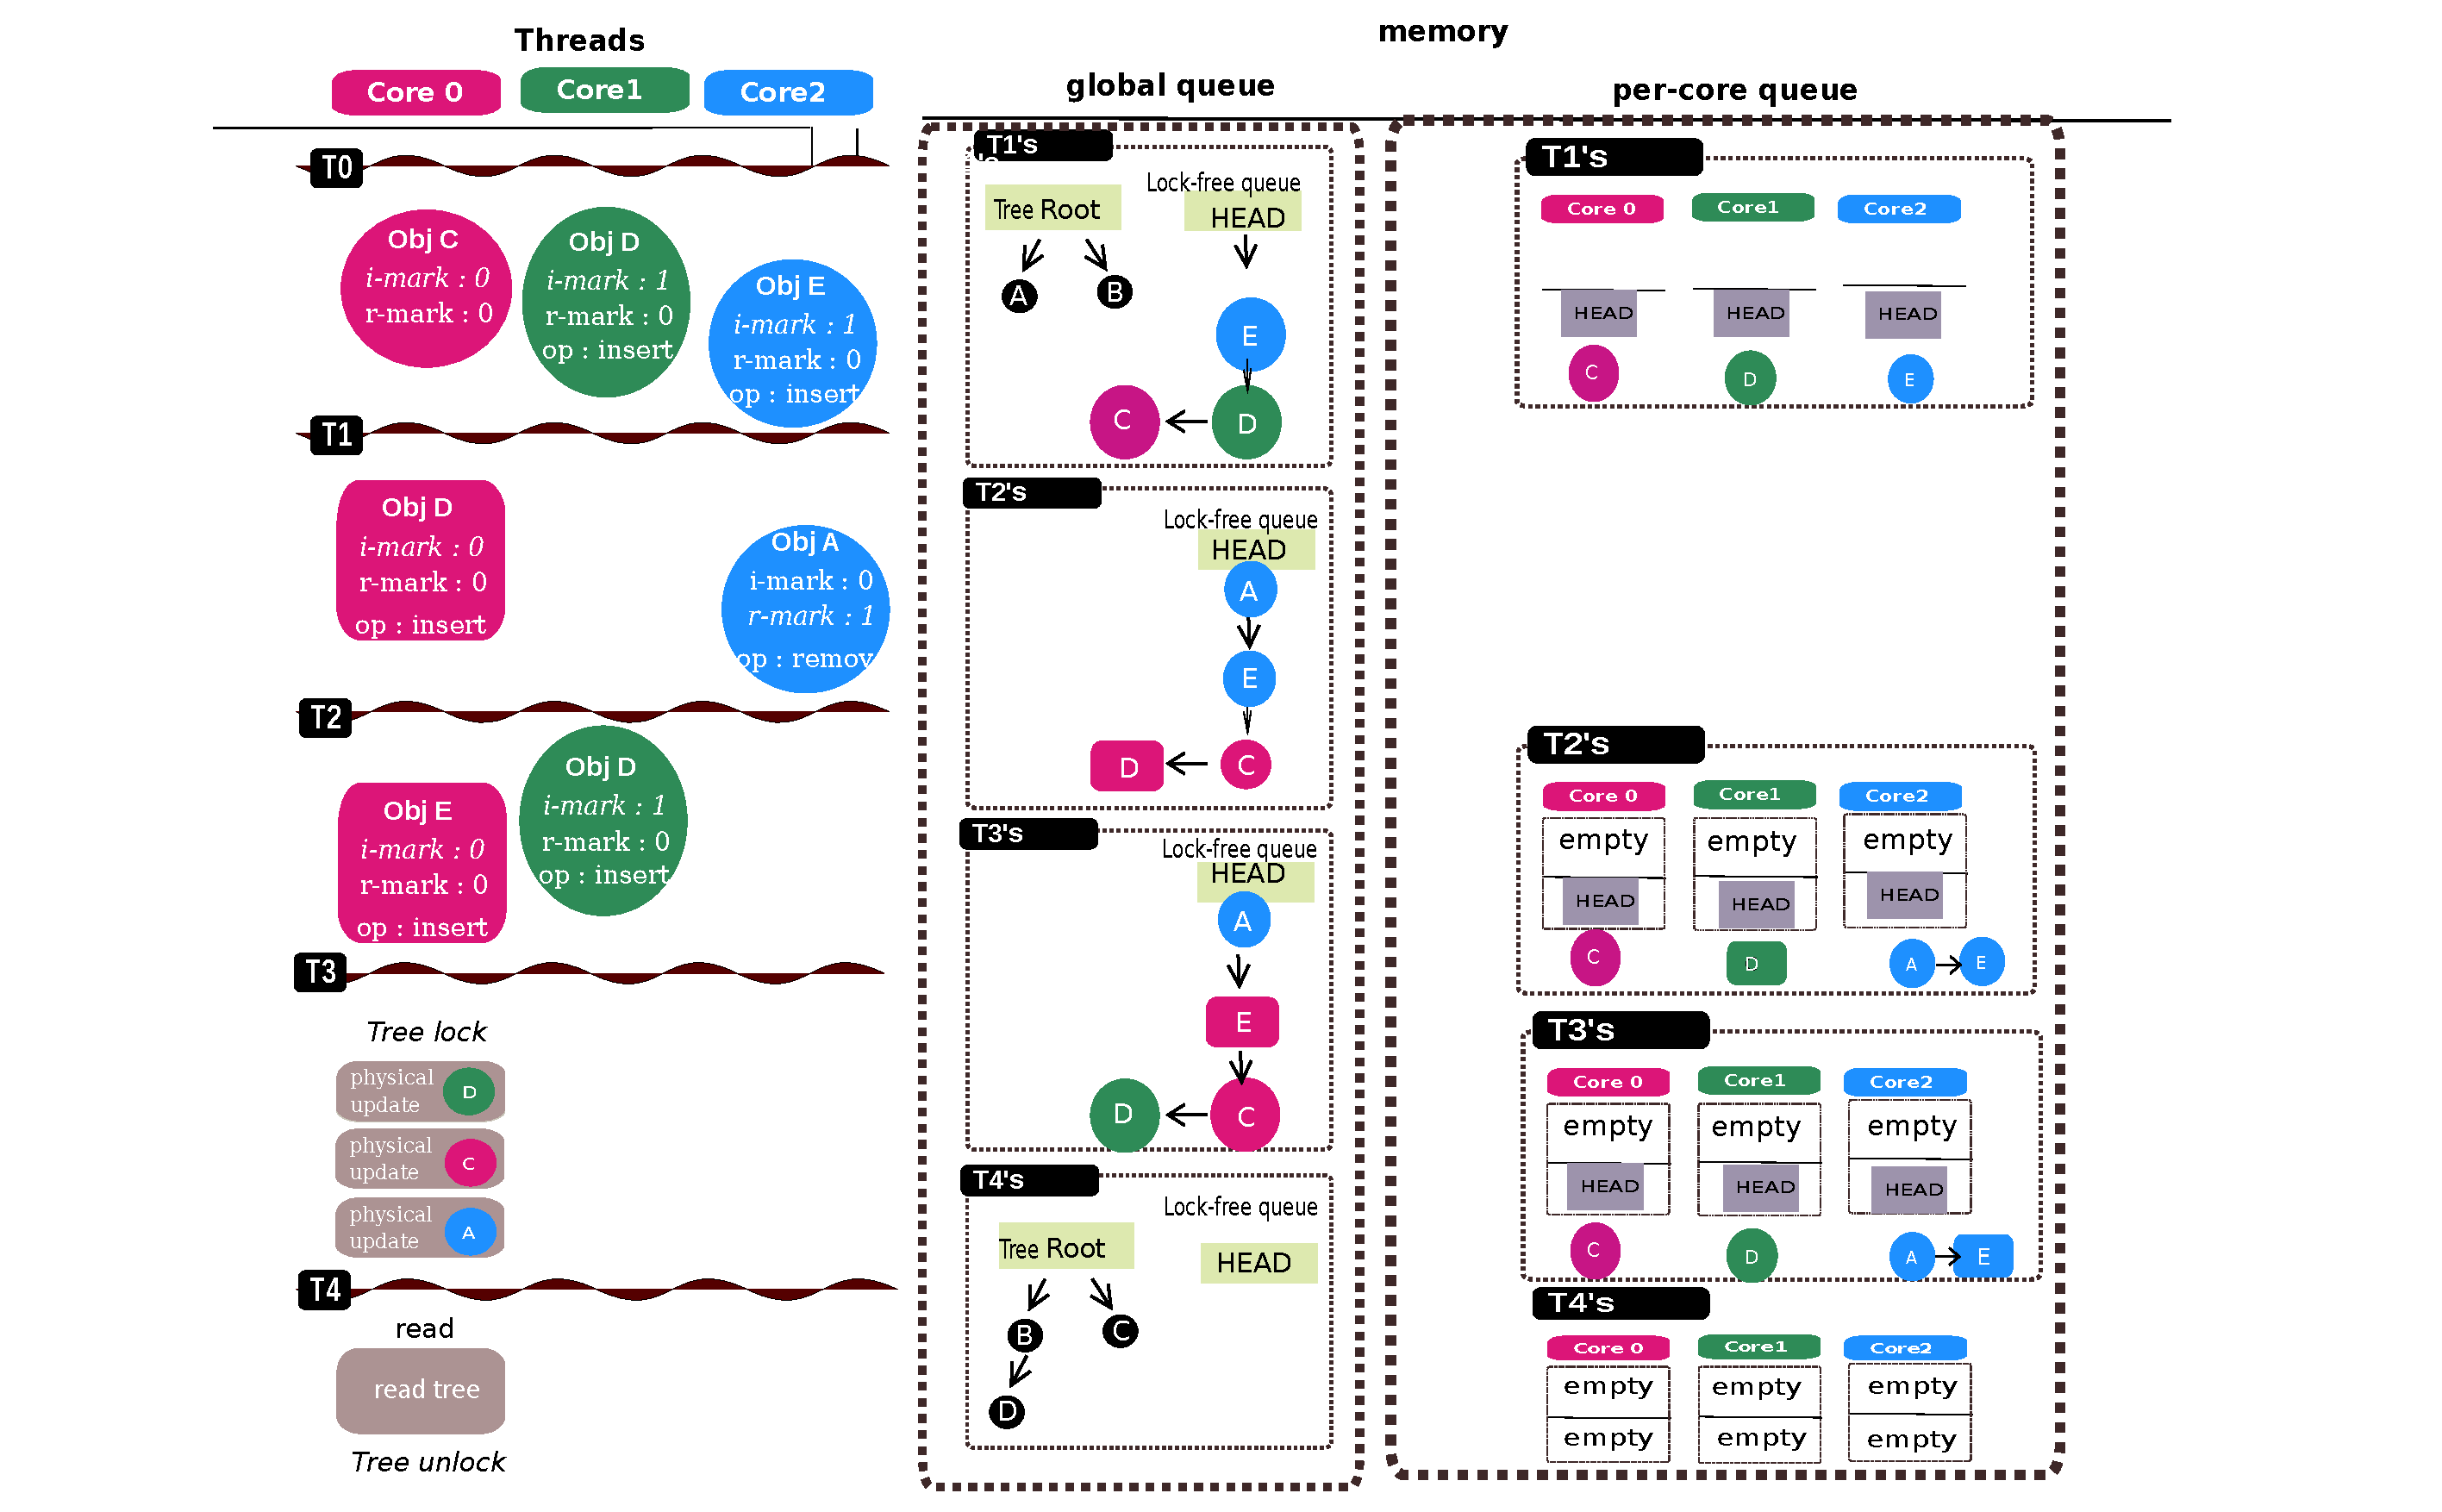
\includegraphics[width=0.5\textwidth,height=0.5\textheight,keepaspectratio]{fig/basic_gldu}
  \end{center}
  \caption{\deferu example showing six update operations and one read
  operation. The execution flows from top to bottom. Memory represents original
  data structure and logging queue at T1, T2 and T3, respectively.}
  \label{fig:basic}
\end{figure}


\ifkor
먼저 LDU를 보다 정확하게 설명하기위해, 로그를 global queue 저장한 방법과 per-core queue에 저장한 두가지 방법에 대해서
예를 들어 설명한다. 
그림 \ref{fig:basic} LDU의 하나의 예에 대해서 보여준다. 그림 \ref{fig:basic}은 예로서 queue를 global
queue를 사용하였다. 6개의 update operation과 1개의 read operation을 LDU에서 어떻게 처리하는지 보여준다.
update operation에 대해서는 앞에서 설명한 심볼을 사용했고 garbage object을 위한 심볼이 추가 되었다.
garbage object는 \res{1}{D}과 같이 rectangle로 표시한다. 
이 그림의 실행 순서는 위에서 부터 아래이다.
그림의 왼쪽은 CPU의 operation 순서를 보여주고 오른쪽은 특정 시간에 메모리에 저장된 자료구조의 내용을 보여준다.
초기 data structure의 트리에는 \inv{0}{A} and \inv{0}{B} 두개의 오브젝트가 들어가고, global
queue에는 아무것도 없다.

그림 \ref{fig:basic}는 시간 순서대로 각단계에 대해서 LDU의 수행 흐름을 보여준다.
먼저 그림에서 concurrent updates 단계에서는 \code{Core0}, \code{Core1} and \code{Core2}가 각각
$\oplus$\inv{1}{C}, $\oplus$\inv{2}{D} and
$\oplus$\inv{3}{E}에 해당하는 3개의 updates oepration을 log로 저장한다. 
Log를 저장하는 queue를 non-blocking queue를 사용하기 때문에, 이 단계에서의 update는 lock이 필요없다. 
즉 모든 thread는 lock에 대한 contention없이 병렬적으로 실행된다. 
\code{T1} 시점이 되면 메모리의 트리는 \inv{0}{A} and \inv{0}{B}의 노드를 가지게 되고, queue에는 
$\oplus$\inv{1}{C}, $\oplus$\inv{2}{D} and $\oplus$\inv{3}{E}가 insert mark 필드가
true로 된 상태로 저장되어 있다. 
update-side absorbing 단계에서는  $\ominus$\inv{1}{D}명령이 수행되면, 새로운 object를 queue에 넣지
않고, mark 필드만 atomic하게 true로 수정한다.  
만약 처음 수행되는 $\ominus$\inv{3}{A} operation이면 queue에 넣는다.
\code{T2} 시점이 되면 메모리의 트리는 변함없고, queue에는 
$\oplus$\inv{1}{C}, $\oplus$\res{2}{D}, $\oplus$\inv{3}{E} and 가
$\ominus$\inv{3}{A} 저장된다. 여기서 \res{2}{D}는 mark필드가 false로 되어 garbage가 된 object이다.
reuse garbage log 단계에서는 \res{2}{D}와 같이 queue에는 들어가 있지만, garbage object인 경우 새롭게
queue에 operation log를 넣지 않고, mark 필드 변경으로 재사용하는 것이다. 
따라서 \res{2}{D}는 \inv{2}{D} 상태로 변경된다. 
\code{T3} 시점이 되면 queue에는 
$\oplus$\inv{1}{C}, $\oplus$\inv{2}{D}, $\oplus$\res{3}{E} and 가
$\ominus$\inv{3}{A} 저장된다.
마지막 단계인 저장된 log를 실행하는 단계에서는 tree에서 사용한 방법으로 lock를 건후 하나의 코어에서 
전체 로그를 update한다. 여기서 garbage log인  $\oplus$\inv{2}{D}을 제외하고 queue에 저장된 순서대로 
$\oplus$\inv{1}{C},$\oplus$\res{3}{E} and 가 $\ominus$\inv{3}{A}의 operation을
수행한다. \code{T4} 시점이 되면 tree에는 
모든 operation이 수행되어, \inv{0}{B}, \inv{0}{C} and \inv{0}{D} 값이 존재하게 된다.
결국 로그를 모두 수행하면 마지막 reader는 같은 tree의 값을 읽게 된다. 

\begin{figure}[tb]
  \begin{center}
     \includegraphics[width=0.5\textwidth,keepaspectratio]{fig/basic_pldu2}
  \end{center}
  \caption{PLDU The execution flows from top to bottom. Memory
  represents original data structure and logging queue at T1, T2 and T3, respectively.}
  \label{fig:basicpldu}
\end{figure}

그림 \ref{fig:basicpldu}는 per-core queue에 log를 저장되는 흐름을 설명한다.
global queue와의 차이점만 설명하면,


\else

\fi

\subsection{The LDU Algorithm}
\begin{figure}[tb!]
\inputminted[linenos,fontsize=\footnotesize, tabsize=2]{c}{src/ldu_logical.c}
\rule{\columnwidth}{0.5pt}
\vspace{-\baselineskip}
\caption{\deferu logical update algorithm. \code{logical\_insert} represents
 non-blocking insert function.
It may be called by original insert position without locks. The fastpath is
 that when their object was removed by \code{logical\_remove},
 \code{logical\_insert} just changes node's marking field.}
\label{fig:gldulogicalupdate}
\end{figure}

\subsubsection{logical update: inserting logs}
%$$$$$$$$$$$$$$$$$$$$$$$$$$$$$$$$$$$$$$$$$$$$$$$$$$$$$$$$$$$$$$$$$$$$$$$$$$$$$$$$
%Paragraph 1:LDU Concurrent Updates 알고리즘 코드 및 설명 
%$$$$$$$$$$$$$$$$$$$$$$$$$$$$$$$$$$$$$$$$$$$$$$$$$$$$$$$$$$$$$$$$$$$$$$$$$$$$$$$$
\ifkor

그림 \ref{fig:gldulogicalupdate}는 concurrent updates를 수행하는 코드와 앞에서 설명한 update-side
absorbing logs와 reuse garbage logs에 대한 코드이다. \code{logical\_insert}과
\code{logical\_remove}의 코드에서 가장 먼저하는 것은 이미 update operation이 수행되어 log가 queue에 들어
있는지에 대해서 체크를 한다. 이것은 update함수가 수행하는 도중 어느때나 log를 flush하는 \code{synchronize} 함수가
수행 될 수 있기 때문에, \code{xchg} 함수를 통해 atomic하게 체크를 한다. 또한 \code{xchg}를 통해 old mark
필드가 true라면 이미 queue에 log가 있다는 뜻이므로, atomic하게 false로 수정을 한다.
이것은 앞에서 설명한 update-side absorbing log 기능이며, 1개의 atomic operation으로 update를 수행할 수
있다.
만약 mark 필드카 체크되지 않았다면, 두번째로 queue에 존재하는 로그인지 체크를 한 후, 존재하는 로그라면
이미 앞에서 mark필드를 설정하여 이미 로그를 재활용했으므로 queue에 로그를 넣지 않는다.
만약 처음 사용된 log라면 non-blocking queue에 넣는다.
이 코드는 항상 옳게 동작한다.  
그 이유는 리눅스 update operation이 항상 insert-remove 순서나 remove-insert 순서로 실행되기 때문이다.
%만약 순서가 insert-insert 또는 remove-remove로 동작하면 
\else

\fi


\subsubsection{physical update: applying logs}


\begin{figure}[tb!]
\inputminted[linenos,fontsize=\footnotesize, tabsize=2]{c}{src/ldu_physical.c}
\rule{\columnwidth}{0.5pt}
\vspace{-\baselineskip}
\caption{\deferu physical update algorithm. \code{synchronize\_ldu} may be
 called by reader and converts update log to original data structure
 traversing the lock-less list.}
\label{fig:glduphysicalupdate}
\end{figure}
%$$$$$$$$$$$$$$$$$$$$$$$$$$$$$$$$$$$$$$$$$$$$$$$$$$$$$$$$$$$$$$$$$$$$$$$$$$$$$$$$
%Paragraph 2:LDU Deferred Updates 알고리즘 코드 및 설명 
%$$$$$$$$$$$$$$$$$$$$$$$$$$$$$$$$$$$$$$$$$$$$$$$$$$$$$$$$$$$$$$$$$$$$$$$$$$$$$$$$

\ifkor
그림 \ref{fig:glduphysicalupdate}는 concurrent updates를 통해 저장된 log들을 적용하는 deferred
update 함수에 대한 코드이다.
\code{synchronize\_ldu}는 마치 CoW 처럼 read 전에 호출되기도 하지만, 로그가 쌓이는것을 방지하기 위해 주기적으로
호출되어 로그를 비워준다.
이 함수는 항상 object의 lock이 걸린 상황에서 수행된다. 
LDU는 single consumer가 독점적으로 log를 처리한다.
따라서 제일 먼저 하는일은 queue에 저장된 log를 얻기 위해 atomic xchg operation으로 log의 head 포인터를
얻는다.
그리고 이 순간 부터는 single consumer가 독점적으로 log를 처리하게 된다.
LDU는 주기적으로 log를 비워줘야 하므로, update operation이 수행되는 도중에도 \code{synchronize\_ldu}가
호출될 수 있다.
따라서 항상 origianl data structure에 적용하기 전에 mark 필드를 초기화해야한다.
또한 log를 사용했으면, used 비트를 초기화 하여 해당 log가 queue 없음을 표시한다.
하지만 mark 필드 초기화 과정과 used 비트를 초기화 하는 과정에서, reuse garbase logs 기능 때문에,
언제든지 다시 concurrent updates operation을 통해 mark 필드가 설정될 수 있다.
따라서 한번 더 mark 필드를 체크하여 log를 비워준다.
\else

\fi

\subsubsection{LDU queues}
\begin{figure}[tb!]
\inputminted[linenos,fontsize=\footnotesize, tabsize=2]{c}{src/ldu_queue.c}
\rule{\columnwidth}{0.5pt}
\vspace{-\baselineskip}
\caption{\deferu physical update algorithm. \code{synchronize\_ldu} may be
 called by reader and converts update log to original data structure
 traversing the lock-less list.}
\label{fig:lduqueue}
\end{figure}

\ifkor
LDU의 로그를 저장하기 위한 2가지 queue에 대한 코드는 그림 \ref{fig:lduqueue}와 같다. 
앞에서 설명했듯이 LDU는 어떤 queue를 사용해도 문제 없도록 설계하였다.
따라서 queue 대한 의존성이 없다.
global queue를 사용할 경우 LDU는 항상 head의 first 포인터에 CAS연산으로 성공할 때까지 반복 수행 후 데이터를 넣는다. 
per-core queue를 사용할 경우는 per-core의 hash 테이블을 가지고 온 후 hash 테이블이 넣으려는 log의
data structure와 같은지 체크하고, 다르면 해당 코어에 저장된 log를 lock과 함께 update를 수행한다.
전체 코어의 log를 flush할 필요없이 해당 코어에 저장된 log만 flush하면 되는 이유는 이미 update-side absorbing에
의해 time-sencitive한 operation이 삭제되었기 때문이다.

\else

\fi




%$$$$$$$$$$$$$$$$$$$$$$$$$$$$$$$$$$$$$$$$$$$$$$$$$$$$$$$$$$$$$$$$$$$$$$$$$$$$$$$$
%Reference Sentence 1
%$$$$$$$$$$$$$$$$$$$$$$$$$$$$$$$$$$$$$$$$$$$$$$$$$$$$$$$$$$$$$$$$$$$$$$$$$$$$$$$$

\ifkor
\else
* By default OpLog executes logged updates in temporal order. For example,
consider a linked list. If a process logs an insert operation on one core,
migrates to another core, and logs a remove operation, the remove should
eventually execute after the insert.
* OpLog relies on timestamps from a system-wide synchronized clock to tell it
how to order entries in different cores' log.
*This ordering ensures linearizaility, making OpLog compatible with existing
data structure semantics.
\fi



%$$$$$$$$$$$$$$$$$$$$$$$$$$$$$$$$$$$$$$$$$$$$$$$$$$$$$$$$$$$$$$$$$$$$$$$$$$$$$$$$
%Reference Sentence 1
%$$$$$$$$$$$$$$$$$$$$$$$$$$$$$$$$$$$$$$$$$$$$$$$$$$$$$$$$$$$$$$$$$$$$$$$$$$$$$$$$

%To keep the log from growing without end, we can at any point apply in-order a
%subsequence of the operations at the head of the log to the state to derive a
%new state, and remove these operation from the log[EuroSys 2006 PLS].

%High level operations performed on shared data structures can be divided into
%three groups: read-only, write-only, and read-modify-write[PLS].

%Read-only operations do not mutate the data, write-only operations modify the
%data but do not return a result, and read-modify-write operations change shared
%data and return a result that is dependent on the data read[PLS].

%Both suffer from a complete loss of scalability beyond a rather low concurrency
%level, because all threads must succesfully apply a CAS operation to the shared
%head or tail of the queue in order to complete their operation[FC].


%$$$$$$$$$$$$$$$$$$$$$$$$$$$$$$$$$$$$$$$$$$$$$$$$$$$$$$$$$$$$$$$$$$$$$$$$$$$$$$$$
%Reference Sentence 2:LDU paper
%$$$$$$$$$$$$$$$$$$$$$$$$$$$$$$$$$$$$$$$$$$$$$$$$$$$$$$$$$$$$$$$$$$$$$$$$$$$$$$$$

%This section describes the \deferu algorithm, a lightweight concurrent
%update for update-heavy data structures based on deferred updates.
%Challenges to designing a deferred update mechanism includes 
%performing concurrent update with minimal
%cache line transfers allowing parallel updates.
%At each update operation, \deferu records this update
%operation log to lock-less list.
%Before the read operation, \deferu applies the updates log in chronological
%order.
%In order to deferred update, \deferu divide the update operation 
%into \emph{logical update} and
%\emph{physical update}.
%The \emph{logical update} inserts logs into the lock-less list and carries out
%update side absorbing; on the other hand, the \emph{physical update} executes
%these operations that are minimized by the update side absorbing.

%\begin{figure}[tb]
%  \begin{center}
    %
    % 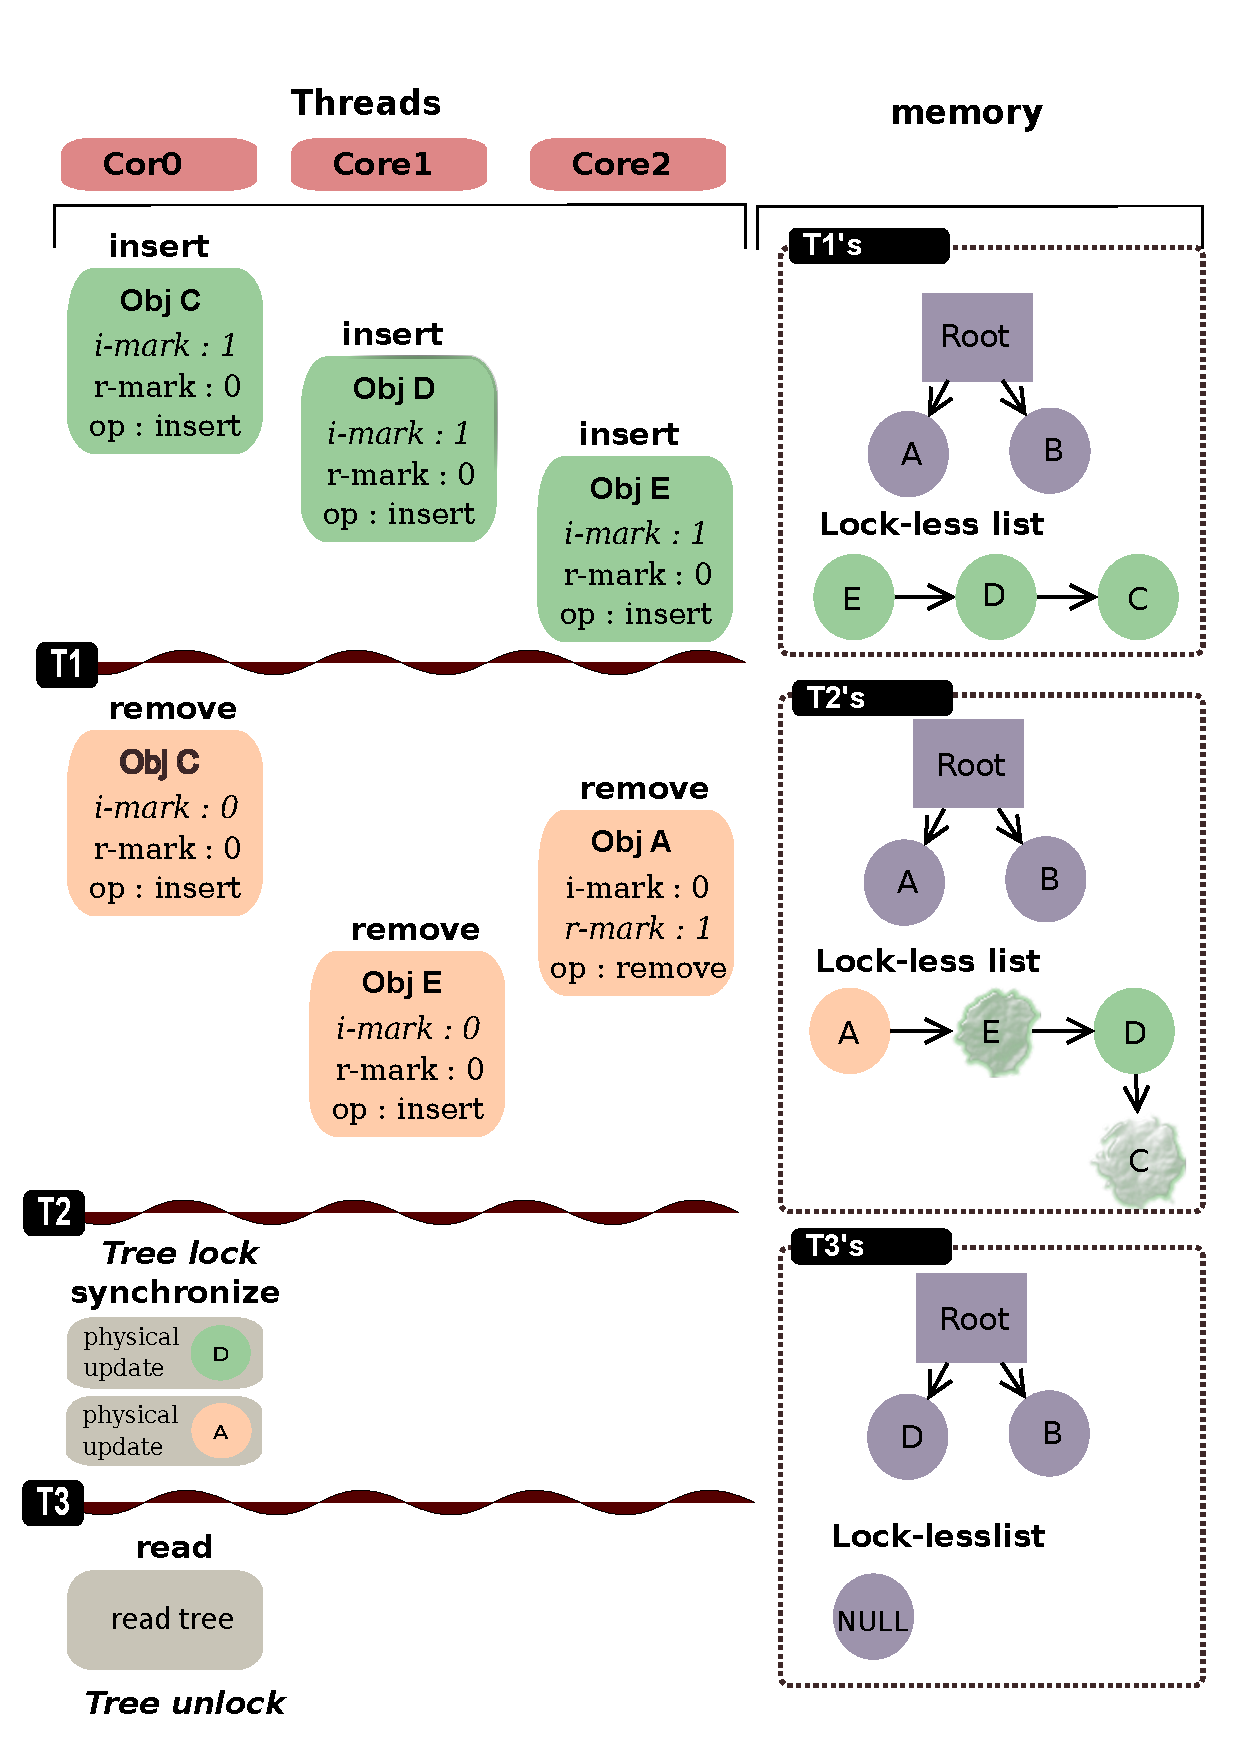
\includegraphics[width=0.5\textwidth,height=0.5\textheight,keepaspectratio]{fig/basic}
%  \end{center}
%  \caption{\deferu example showing six update operations and one read
%  operation. The execution flows from top to bottom. Memory represents original
%  data structure and logging queue at T1, T2 and T3, respectively.}
%  \label{fig:basic}
%\end{figure}

%\subsection{Approach}

%\deferu's scheme for concurrent update is proposed to overcome limitations
%of Linux kernel where 
%both insert and remove operations must not be invoked concurrently for the same
% object, but reads can be concurrently invoked with update.
%\deferu borrows ideas from Oplog's deferred processing and Harris' marking
% scheme.
%The reason is that Linux kernel's object management scheme differs from
% research-oriented data structure such as the lock-free and wait-free data
% structures~\cite{Harris2001Lockfree}~\cite{Fomitchev2004Lockfree}~\cite{Timnat2012}.
%For example, consider the Harris linked list, an insert operation inserts an 
%integer key into the data structure, but Linux kernel inserts their object link.
%The Linux kernel's list operations do not depend on key value.
%Furthermore, Harris linked list node's constructor can be invoked
%upon the insert function's scope, but Linux kernel's node is created on outside scope.
%In this regard, if duplicated remove operation occur, the Linux kernel may
%fail because their link pointer had been freed from destructor.
%Therefore, if a operation is an insert operation, the after operation must occurs 
%remove operation with regard to same object;the remove must execute after the 
%insert, or insert must execute after the remove.
%It means that updates such as insert and remove must not concurrently occur at
%the same object, but reads can occur concurrently.
%\deferu scheme inspires by this operation sequence, and inherits ideas
%from Oplog's deferred processing and Harris's marking scheme.

%\deferu's scheme for concurrent update inspires by Linux kernel's operation
%sequence.
%For example, consider a linked list in Linux kernel, if a operation is an insert
%operation, the after operation must occurs remove operation because Linux
%kernel's object management scheme differs from research-oriented data structure
%such as the lock-free and wait-free data
%structures~\cite{Harris2001Lockfree}~\cite{Fomitchev2004Lockfree}.
%Linux kernel's list operations do not depend on key value, but their 
%list operations depend on their object.
%These structure are their node's constructor can be invoked upon the insert
%function's scope, but Linux kernel's node is created on outside scope.
%In this regard, if duplicated remove operation occur, the Linux kernel may
%fail because their link pointer had been freed from destructor.
%Therefore, the remove must execute after the insert, or insert must execute
%after the remove.
%It means that updates such as insert and remove cannot concurrently occur at
%the same object, but reads can occur concurrently.
%\deferu scheme inspires by this operation sequence, and inherits ideas
%from Oplog's deferred processing and Harris's marking scheme.

%One important algorithm in our proposed novel concurrent update scheme is
%update-side absorbing operation that cancels duplicated operations for
% optimizations.
%A new remove operation, for example, may cancel an existing insert operation
%with regard to same object, so reader can eventually reads consistent data.
%Even though the Oplog's absorbing operation is invoked by
%read, \deferu's absorbing operation is fully invoked by update, so read-side
%performance is enhanced.

%The basic principle of update-side absorbing is that update uses atomic 
%marking operation for the object's mark field, which allows previous operation
% to cancel.
%For instance, if a new remove operation occurs after insert operation of the
%same object, \deferu does not store this operation in the lock-less
%list; instead, it changes the insert mark field to zero using the CAS.
%This mark is checked later when reading operation occurs and the operation log 
%maintained in the lock-less list is applied to original data structure
% atomically.
%This action may give effective update;however, the inserted operation log has
% remained in the lock-less list, so \deferu's reader checks the mark field
% when they convert operation log to original data structure atomically.

%figure : basic principle 
%Figure \ref{fig:basic} gives an example of deferred update with six update
%operations and one read operation.
%In this figure, execution flows from top to bottom.
%The data structure for \emph{physical update} is a tree, and initial values in
%the tree are node \code{A} and \code{B}.
%In contrast, the data structure for \emph{logical update} is lock-less list.
%In the top figure, \code{Core0}, \code{Core1} and \code{Core2} perform the
%logical insert operation to nodes \code{C}, \code{D} and \code{E},
% respectively.
%The logical inserts set the insert mark, and they then insert their
%nodes into lock-less list.
%In this case, none of the lock is needed because \deferu uses the lock-less
%list;all threads can execute the update concurrently.
%At \code{T1}, the tree contains node \code{A}
%and \code{B} and 
%the lock-less list contains node \code{E}, \code{D} and \code{C}.
%When removing the node \code{C}, the node \code{C}, whose mark field was marked
%by insert, atomically cleans up the insert marked field.
%At \code{T2}, the lock-less list contains nodes
%\code{A}, \code{E}, \code{D}, and \code{C}, and the marking field is zero for 
%nodes \code{E} and \code{C}.
%Before running the \code{synchronize} function, they need to lock the original
% tree's lock using the exclusive lock in order to protect the tree's
% operation.
%The \code{synchronize} migrates from lock-less list node to tree node, each of 
%which is the marked node, so nodes \code{A} and \code{D} are migrated.
%Finally, the tree contains nodes \code{D} and \code{B}, so the reader can read
% eventually consistent data.

%First, removing the cancelable operation at update point, \deferu uses the
% update side absorbing instead of read before absorbing.
%Therefore, read before operations in \deferu are fast because read-side
%absorbing operation is eliminated. 
%One notable difference between Oplog and \deferu is that 
%\deferu uses a light weight global queue with non-blocking synchronization 
%for update logs and eliminates time stamps while Oplog is dependent on 
%per-core logs with time stamps.
%By eliminating the global time stamps(hardware-dependent feature), \deferu is
% not dependent on hardware feature.
%Furthermore, update operations in \deferu are also fast because they use
%efficient update-side absorbing that eliminates traversal finding the
%cancelable operation.
%Furthermore, to optimize the log management and minimize the traversal
% overheads during reading, \deferu applies efficient update-side absorbing
% algorithm instead of read-side absorbing algorithm.

%\subsection{logical update}
%\begin{figure}[tb]
%\begin{obeylines}
%\begin{obeyspaces}
%function \(logical\_insert(obj, root) \):
%~~~If CAS(obj.del\_node.mark, 1, 0) $\ne$ 1:  
%~~~    obj.add\_node.mark $\gets$ 1
%~~~    If test\_and\_set\_bit(OP\_INSERT, obj.exist) $\ne$ true:
%~~~        set\_bit(OP\_INSERT, obj.used):
%~~~        obj.add\_node.op $\gets$ OP\_INSERT
%~~~        obj.add\_node.key $\gets$ obj
%~~~        obj.add\_node.root $\gets$ root
%~~~        add\_lock\_less\_list(obj.add\_node)
%~~~
%~~~
%function \(logical\_remove(obj, root) \):
%~~~If CAS(obj.add\_node.mark, 1, 0) $\ne$ 1:  
%~~~    obj.del\_node.mark $\gets$ 1 
%~~~    If test\_and\_set\_bit(OP\_REMOVE, obj.exist) $\ne$ true:
%~~~        set\_bit(OP\_REMOVE, obj.used):
%~~~        obj.del\_node.op $\gets$ OP\_REMOVE
%~~~        obj.del\_node.key $\gets$ obj
%~~~        obj.del\_node.root $\gets$ root
%~~~        add\_lock\_less\_list(obj.del\_node)

%\end{obeyspaces}
%\end{obeylines}
%\rule{\columnwidth}{0.5pt}
%\vspace{-\baselineskip}
%\caption{\deferu logical update algorithm. \code{logical\_insert} represents
% non-blocking insert function.
%It may be called by original insert position without locks. The fastpath is
% that when their object was removed by \code{logical\_remove},
% \code{logical\_insert} just changes node's marking field.}
%\label{fig:logicalupdate}
%\end{figure}

%The pseudo code for \deferu's \emph{logical update} is given in
%figure~\ref{fig:logicalupdate}.
%The \code{logical\_insert}, the concurrent update function, checks whether this
%object already has been removed by \code{logical\_remove}.
%If this object has been removed, \code{logical\_insert} initializes the marking
% field and then they return, which is fastpath.
%The marking field needs synchronization because this field in the
%\emph{logical update} is shared with the \emph{physical update}, so the CAS
% operation is needed.
%When the marking field has been initialized, they set the
%marking field, then they check whether or not this node already has been
% inserted in lock-less list.
%If the node does not exist in lock-less list, then they insert the node into
%lock-less list.

%\subsection{Physical update}
%\begin{figure}[tb]
%\begin{obeylines}
%\begin{obeyspaces}
%function \(synchronize\_ldu(obj, head) \):
%~~~If (head.first = NULL): 
%~~~    return; 
%~~~entry $\gets$ xchg(head.first, NULL);
%~~~for each list node:
%~~~    obj $\gets$ node.key
%~~~    clear\_bit(node.op, obj.exist)
%~~~    If CAS(node.mark, 1, 0) = 1:
%~~~         physical\_update(node.op, obj, node.root)
%~~~    clear\_bit(node.op, obj.used)
%~~~
%function \(physical\_update(op, obj, root) \):
%~~~If op = OP\_INSERT :  
%~~~    call real insert function(obj, root) 
%~~~Else If op = OP\_REMOVE :  
%~~~    call real remove function(obj, root) 

%\end{obeyspaces}
%\end{obeylines}
%\rule{\columnwidth}{0.5pt}
%\vspace{-\baselineskip}
%\caption{\deferu physical update algorithm. \code{synchronize\_ldu} may be
% called by reader and converts update log to original data structure
% traversing the lock-less list.}
%\label{fig:physicalupdate}
%\end{figure}

%The pseudo code for \deferu's \emph{physical update} is given in
%Figure~\ref{fig:physicalupdate}.
%First, they check whether lock-less list is an empty list or not, then they
%iterate the lock-less list.
%If the marking field has been set, they execute migration from
%lock-less to original data structure.
%Because the marking field in \emph{physical update} is shared with
% \emph{logical update}, the CAS operation is needed.
%They initialize the used field, which needs to protect the object from freed
% through destructor.
%The programmer must acquire locks on the \code{synchronize\_ldu} function,
%which migrates log to original data structure.
%Finally, the \code{physical\_update} executes original functions by using the
%operation log.

\section{Concurrent updates for Linux kernel}

\subsection{Case study:reverse mapping}

%$$$$$$$$$$$$$$$$$$$$$$$$$$$$$$$$$$$$$$$$$$$$$$$$$$$$$$$$$$$$$$$$$$$$$$$$$$$$$$$$
%Paragraph 1: Linux의 reverse mapping에 대한 자세한 설명 
%$$$$$$$$$$$$$$$$$$$$$$$$$$$$$$$$$$$$$$$$$$$$$$$$$$$$$$$$$$$$$$$$$$$$$$$$$$$$$$$$
리눅스 커널의 프로세스간 공유자원 중 하나인 reverse page mapping(rmap)은 fork, exit, mmap이 수행될 때
update가 많이 발생하는 data structure이다.
Linux's reverse mapping reads walked through each process’s pages mappings and
selected pages to unmap when it swaps a pyhsical page out to disk, migrates
other cpu, or turncates a file.
After all a page’s mappings were removed could it be selected for
pageout~\cite{OBJMAPOLS}.
Rmap의 anonymous page와 file page의 관리는 최근 interval trees로 되어 있으며, 이것은 reverse page
성능 향상으로 위해 지속적으로 최적화가 ~\cite{CorbetLWNRMAP}~\cite{CorbetLWNANON} 이루어지고 있다. 

리눅스는 rmap의 interval tree를 보호하기 위해 rw semapore를 사용한다. 
따라서, 프로세스들이 fork, exit, mmap를 simultaneosly 수행하면 interval tree를 보호하는
read-write semapore 때문에 scalability가 떨어진다.
anonymous page를 위한 rmap과 file mapped page을 위한 rmap 모두 문제가 있다.
이번 장은 이러한 문제를 해결하기 위해, 어떻게 LDU를 리눅스의 rmap에 적용했는지에대한 내용을 설명하며, 보다 practial한 내용을
다룬다.

%The Linux rmap implementation can become a bottleneck when many processes
% simultaneously try to map the same file.
%For exemaple, simultaneous creation of many processes is likely to cause
% contention for the lock protecting the interval tree of the libc library,

%Objmap
%rmap is a mechanism for translating physical addresses to user virtual
% addresse.
%commonly called reverse mapping, or rmap. 
%This meant it was not possible for the memory management subsystem to point to
% a physical page and remove all its mappings. 
%There was a mechanism that walked through each process’s mappings and selected
%pages to unmap.
%Only after all a page’s mappings were removed could it be selected for pageout

%Many in the memory management community considered this very inefficient.
%Page aging and removal could be made much more efficient if the page could be
%directly unmapped when it was ready to be removed.
%Some form of rmap was clearly needed for this to work.

%Oplog
%Linux's reverse map(ramp) records, for each physical page, all page table
% entries that map that page.
%Linux reads these reverse mappings when it truncates a file or swaps a physical
% page out to disk, in order to find(and then delete) all page table entries
% that refer to the deleted page(s).
%The fork(), exit(), and mmap() system calls update the rmap, but don't need to
% read it.
%The Linux designers have heavily optimized the rmap using interval
% trees[21, 22, 24].
%Each file has an associated interval tree protected by a lock.
%A file's interval tree maps intervals of the file to virtual address mappings.
%Each virrtual address mapping maps one or more pages from the file.
%The Linux rmap implementation can become a bottleneck when many processes
% simultaneously try to map the same file.
%For exemaple, simultaneous creation of many processes is likely to cause
% contention for the lock protecting the interval tree of the libc library,
% because creating a process entails creating virtual address mappings for libc
% and inserting the mappings into the libc ramp interval tree.


\subsection{anonymous mapping}

\begin{figure}[tb]
  \begin{center}
     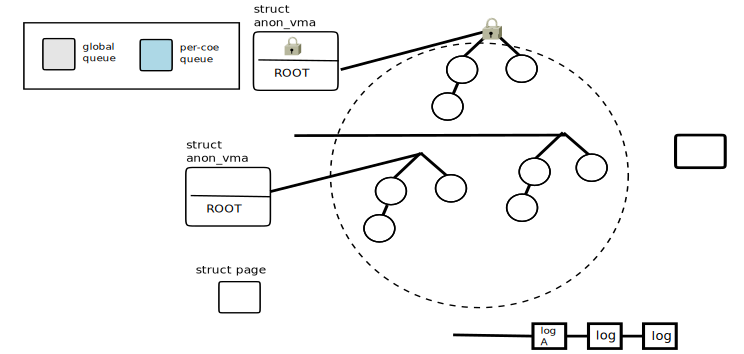
\includegraphics[width=0.5\textwidth,height=0.5\textheight,keepaspectratio]{fig/anon_vma}
  \end{center}
  \caption{An example of applying the \deferu to file reverse mapping. }
  \label{fig:deferu2}
\end{figure}


%$$$$$$$$$$$$$$$$$$$$$$$$$$$$$$$$$$$$$$$$$$$$$$$$$$$$$$$$$$$$$$$$$$$$$$$$$$$$$$$$
%Paragraph 1: linux의 anon vma의 공유된 구조에 대한 설명
%$$$$$$$$$$$$$$$$$$$$$$$$$$$$$$$$$$$$$$$$$$$$$$$$$$$$$$$$$$$$$$$$$$$$$$$$$$$$$$$$
Anonymous rmap의 공유데이터는 서로 상당히 복잡하게 연결되어 있다.
그림 x-x는 이렇게 복잡하게 연결된 공유데이터를 보여준다. 




%$$$$$$$$$$$$$$$$$$$$$$$$$$$$$$$$$$$$$$$$$$$$$$$$$$$$$$$$$$$$$$$$$$$$$$$$$$$$$$$$
%Paragraph 2: anon vma에 ldu 적용한 방법에 대한 설명 
%$$$$$$$$$$$$$$$$$$$$$$$$$$$$$$$$$$$$$$$$$$$$$$$$$$$$$$$$$$$$$$$$$$$$$$$$$$$$$$$$


\subsection{file mapping}

\begin{figure}[tb]
  \begin{center}
     \includegraphics[width=0.5\textwidth,height=0.5\textheight,keepaspectratio]{fig/file_rmap}
  \end{center}
  \caption{An example of applying the \deferu to file reverse mapping. }
  \label{fig:deferu}
\end{figure}


%$$$$$$$$$$$$$$$$$$$$$$$$$$$$$$$$$$$$$$$$$$$$$$$$$$$$$$$$$$$$$$$$$$$$$$$$$$$$$$$$
%Paragraph 1: linux의 file mapped page reverse mapping의 구조에 대한 설명
%$$$$$$$$$$$$$$$$$$$$$$$$$$$$$$$$$$$$$$$$$$$$$$$$$$$$$$$$$$$$$$$$$$$$$$$$$$$$$$$$
file rmap의 공유데이터는 anonymous rmap보다는 덜 복잡하게 연결되어 있다.
그림 x는 file rmap의 공유데이터를 보여준다. 

%The kernel has the information to do object-based reverse mapping for files.
%Each struct page for a file has an offset and a pointer to a struct
%address\_space, which is the base anchor for all memory associated with file. 
%Every time a range of data from that file is mapped to a process, a
%vm\_area\_struct or vma is created.
%The vma contains the virtual address of the mapping and the base offset within
%the file.
%It is then added to a linked list of all vmas in the address\_space for that
%file.

%$$$$$$$$$$$$$$$$$$$$$$$$$$$$$$$$$$$$$$$$$$$$$$$$$$$$$$$$$$$$$$$$$$$$$$$$$$$$$$$$
%Paragraph 2: file mapping에 ldu 적용한 방법에 대한 설명 
%$$$$$$$$$$$$$$$$$$$$$$$$$$$$$$$$$$$$$$$$$$$$$$$$$$$$$$$$$$$$$$$$$$$$$$$$$$$$$$$$
File mapping의 GLDU는 address\_space object이 interval tree의 head를 가지고 있으므로, 그 곳에
operation log저장한다. File mapping의 PLDU는 per-core hash 테이블로 구현하였고, PLDU를 적용하는데 문제가
없다.
그 이유는 상대적으로 log의 header를 가지고 있는 address\_space가 상대적으로 적게 생성이 되어 hash 충돌이 적게 나타나기
때문에 scalability가 떨어지지 않는다.






%$$$$$$$$$$$$$$$$$$$$$$$$$$$$$$$$$$$$$$$$$$$$$$$$$$$$$$$$$$$$$$$$$$$$$$$$$$$$$$$$
%$$$$$$$$$$$$$$$$$$$$$$$$$$$$$$$$$$$$$$$$$$$$$$$$$$$$$$$$$$$$$$$$$$$$$$$$$$$$$$$$
%Reference Sentence 1
%$$$$$$$$$$$$$$$$$$$$$$$$$$$$$$$$$$$$$$$$$$$$$$$$$$$$$$$$$$$$$$$$$$$$$$$$$$$$$$$$




%$$$$$$$$$$$$$$$$$$$$$$$$$$$$$$$$$$$$$$$$$$$$$$$$$$$$$$$$$$$$$$$$$$$$$$$$$$$$$$$$
%Reference Sentence 2:LDU paper
%$$$$$$$$$$$$$$$$$$$$$$$$$$$$$$$$$$$$$$$$$$$$$$$$$$$$$$$$$$$$$$$$$$$$$$$$$$$$$$$$


%Figure : AIM7 실험 결과
%\begin{figure}[tb]
%  \begin{center}
%    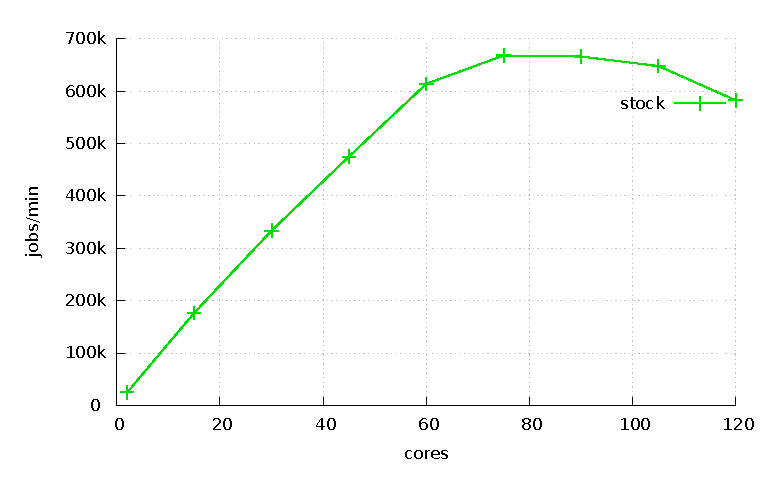
\includegraphics[scale=0.65]{graph/aim7_default.eps}
%  \end{center}
%  \caption{Scalability of AIM7 multiuser. This workload simultaneously create
%  many processes.
%  Up to 60 core, the stock Linux scale linearly, then they flattens out.}
%  \label{fig:aim7_default}
%\end{figure}
 
%In this section, we describe how to apply our concurrent update based on
%deferred update method to Linux.
%The Linux fork is associate with an anonymous page and a file page.
%When many processes are simultaneously created in Linux, 
%these two reverse mapping
%can become bottlenecks since their data structures are shared between
%processes.
%Figure~\ref{fig:aim7_default} shows the scalability problem in case
%of the fork-intensive workload that simultaneously creates many processes.
%Up to 60 core, the stock Linux scales linearly, then creating the reverse
%mapping becomes the bottleneck because their interval trees are protected by
%locks.
%Therefore, fork-intensive workload can pose a scalability bottleneck due to the
%update-heavy data
%structures~\cite{SilasBoydWickizerPth}~\cite{Andi2011adding}~\cite{Tim2013adding}.

%Figure mapped page에 대에 적용한  그림
%\begin{figure}[tb]
%%  \begin{center}
    %
    % \includegraphics[width=0.5\textwidth,height=0.5\textheight,keepaspectratio]{fig/deferu}
%  \end{center}
%  \caption{An example of applying the \deferu to file reverse mapping. }
%  \label{fig:deferu}
%\end{figure}


%Paragraph 6: DeferU 알고리즘 적용 - Mapped page - 리눅스 자료구조를 수정
%Figure~\ref{fig:deferu} gives an example of applying the \deferu to file
%reverse mapping and shows relationship between interval trees and lock-less
% lists.
%An interval tree contains two \code{virtual memory area}(\code{VMA}) nodes; 
%on the other hand, the lock-less list contains the right \code{VMA} as shown in
%Figure~\ref{fig:deferu}.
%It means that the right \code{VMA} has been deleted, and the synchronization
% has not been invoked. 

%In order to using the \deferu, the data structures involved in the
%head(\code{address\_space}) or the node(\code{vm\_area\_structure}) can be
% modified with \deferu's structure as shown in Figure~\ref{fig:deferu}. 
%In addition, programmer must replace \emph{physical update} with \emph{logical
%update} to eliminate the lock. 
%Before the corresponding readers need to be read, \deferu must call synchronize
%function to keep the consistency.

\section{Detail Implementation}\label{sec:implementation}

%$$$$$$$$$$$$$$$$$$$$$$$$$$$$$$$$$$$$$$$$$$$$$$$$$$$$$$$$$$$$$$$$$$$$$$$$$$$$$$$$
%Paragraph 1: 커널 버전 및 코드 분량, 테스트에 대한 설명
%$$$$$$$$$$$$$$$$$$$$$$$$$$$$$$$$$$$$$$$$$$$$$$$$$$$$$$$$$$$$$$$$$$$$$$$$$$$$$$$$
\ifkor
We implemented the new deferred update algorithm in Linux 4.5.rc6 kernel, and
our modified Linux is available as open source. 
global queue를 사용한 버전일 경우 코드의 수정량은 xx-xx을 가지며 덜 복잡한 구조이며, 
percore를 사용할 경우 코드 수정량은 xx-xx을 가진다. 
\else
We implemented the new deferred update algorithm in Linux 4.5.rc6 kernel, and
our modified Linux is available as open source. 
The version of global queue modified code is xx that less complex, but per-core
queue the modified code is xx-xx.
\fi

%$$$$$$$$$$$$$$$$$$$$$$$$$$$$$$$$$$$$$$$$$$$$$$$$$$$$$$$$$$$$$$$$$$$$$$$$$$$$$$$$
%Paragraph 2: per-core queue 구현에 대한 설명 
%$$$$$$$$$$$$$$$$$$$$$$$$$$$$$$$$$$$$$$$$$$$$$$$$$$$$$$$$$$$$$$$$$$$$$$$$$$$$$$$$
\ifkor
LDU percore queue는 2가지 방법으로 구현되었다. 
첫번째 방법은 percore hash table로 구현하는 방법이다.
percore hash table 방법은 direct-mapped cache 처럼 구현하여, 버켓에는 하나의 object만 존재하도록
만든 방법이다. 
만약 hash 충돌이 발생하면 기존 해당 코어의 log를 flush하는 일을 수행한다.
이것은 file reverse mapping 처럼 object가 많이 생기지 않을 때 유용하다. 
이 방법은 기존 코드에 대한 수정없이 적용이 가능하고 추가적인 lock이 필요없다.
하지만 이 방법은 anonymous reverse mapping 처럼 object가 많이 생기는 경우, hash 충돌로 인해 
성능상 오버헤드가 생긴다. 
따라서 anonymous reverse mapping의 percore queue는 percore data에 object별로
구분하지 않고 로그를 저장한 후 실제 percore log를 수행할 때 global lock을 사용하여 보호하였다. 
\else
%LDU percore queue는 2가지 방법으로 구현되었다. 
%첫번째 방법은 percore hash table로 구현하는 방법이다.
The implimentation of per-core queue in the LDU uses per-core hash table that 
can easily distinguish each object.
%percore hash table 방법은 direct-mapped cache 처럼 구현하여, 버켓에는 하나의 object만 존재하도록
%만든 방법이다. 
The LDU per-core hash table implemented as a direct-mapped cache, which one
bucket only has an object because recently used objects will be in the hash
table[Oplog].
%만약 hash 충돌이 발생하면 기존 해당 코어의 log를 flush하는 일을 수행한다.
When this hash table is met a hash conflict, the LDU evits the object in the
hash slot located in the per-core memory.
%이것은 file reverse mapping 처럼 object가 많이 생기지 않을 때 유용하다. 
This method is useful when the number of the root objects is small like the file
rmap(\code{struct address\_space}).
%이 방법은 기존 코드에 대한 수정없이 적용이 가능하고 추가적인 lock이 필요없다.
Moreover, this method reduce additional tasks of programers because it can
minimize code modifications and does not need additional locks.
%하지만 이 방법은 anonymous reverse mapping 처럼 object가 많이 생기는 경우, hash 충돌로 인해 성능상
% 오버헤드가 생긴다.
The per-core hash table, however, incurs a hash conflict overhead.
Since the anonymous rmap creates many of child root object(anon\_vma), so it
incurs a hash conflict overhead.
%따라서 anonymous reverse mapping의 percore queue는 percore data에 object별로 구분하지 않고
% 로그를 저장한 후 실제 percore log를 수행할 때 global lock을 사용하여 보호하였다.
In the case of the anonymous ramp, we do not distinguish object headers to
avoid the hash conflict overhead, but it needs addictional tasks with global
lock.
\fi

%$$$$$$$$$$$$$$$$$$$$$$$$$$$$$$$$$$$$$$$$$$$$$$$$$$$$$$$$$$$$$$$$$$$$$$$$$$$$$$$$
%Paragraph 3: object를 나중에 free하는 내용 설명 
%$$$$$$$$$$$$$$$$$$$$$$$$$$$$$$$$$$$$$$$$$$$$$$$$$$$$$$$$$$$$$$$$$$$$$$$$$$$$$$$$
% 기존 코드를 변경없이 




%$$$$$$$$$$$$$$$$$$$$$$$$$$$$$$$$$$$$$$$$$$$$$$$$$$$$$$$$$$$$$$$$$$$$$$$$$$$$$$$$
%$$$$$$$$$$$$$$$$$$$$$$$$$$$$$$$$$$$$$$$$$$$$$$$$$$$$$$$$$$$$$$$$$$$$$$$$$$$$$$$$
%Reference Sentence 1
%$$$$$$$$$$$$$$$$$$$$$$$$$$$$$$$$$$$$$$$$$$$$$$$$$$$$$$$$$$$$$$$$$$$$$$$$$$$$$$$$








%$$$$$$$$$$$$$$$$$$$$$$$$$$$$$$$$$$$$$$$$$$$$$$$$$$$$$$$$$$$$$$$$$$$$$$$$$$$$$$$$
%Reference Sentence 2:LDU paper
%$$$$$$$$$$$$$$$$$$$$$$$$$$$$$$$$$$$$$$$$$$$$$$$$$$$$$$$$$$$$$$$$$$$$$$$$$$$$$$$$
%\section{Implementation}\label{sec:implementation}
%We implemented the new deferred update algorithm in Linux 3.19.rc4 kernel, and
%our modified Linux is available as open source.
%\deferu's scheme is based on deferred processing, so it needs a garbage
%collector for delayed free.
%In order to implement the garbage collector, we use the lock-less list and a
%periodic timer(1 sec) in the Linux.

%Paragraph 2: 문제점을 해결하기 위해 Harris linked list를 적용
%We compare our \deferu implementation to a concurrent non-blocking Harris
%linked list ~\cite{Harris2001Lockfree};therefore, we implement the Harris
%% linked list to Linux kernel.
%The code refers from sysnchrobench~\cite{Gramoli2015Synchrobench} and
%ASCYLIB~\cite{David2015ASYNCHRONIZED}, and we convert their linked list to
%Linux kernel style.
%Because both synchrobench and ASCYLIB leak memory, we implement additional
%garbage collector for the Linux kernel using Linux's work queues and lock-less
%list.

%Paragraph 3: 오브젝트의 특징을 고려한 lock-free list 구현 
%In order to further improve performance, we move their ordered list to
%unordered list. 
%A feature of the Harris linked list is all the nodes are ordered by
%their key. 
%Zhang~\cite{zhang2013practical} implements a lock-free unordered list
%algorithm, whose list is each insert and remove operation appends an
%intermediate node at the head of the list;these approach is practically
%hard to implement.
%Indeed, Linux does not require contains operation because the Linux data
%structures such as list, tree and hash table not depended on search key;they
%depend on their unique object.
%This feature can eliminates the ordered list in Harris linked list.
%Therefore, we perform each insert operation appends an intermediate node at
%the first node of the list;on the other hand, each remove operation searches
%from head to their node.

%Paragraph 4: mapping은 DeferU와 Harris linked 리스트 둘 다 적용, 
%하지만 anon은 Harris Lined list 만 적용과 이유
%To the scalability of fork, the reverse mapping's lock contention should
%be eliminated not only from file reverse mapping but also from anonymous
% reverse mapping.
%The structure of file reverse mapping is simplified relatively to the
%structure of anonymous mapping because the anonymous reverse mapping is
%entangled by their global object(\code{anon\_vma}) and their
%chain(\code{anon\_vma\_chain});therefore, we only apply \deferu to file reverse
%mapping.


\section{Evaluation}

This section answers the following questions experimentally:
\begin{CompactItemize}
\item Does \ldu's design matter for applications?

\item Why does \ldu's scheme scale well?
\end{CompactItemize}


\subsection{Experimental setup}
%$$$$$$$$$$$$$$$$$$$$$$$$$$$$$$$$$$$$$$$$$$$$$$$$$$$$$$$$$$$$$$$$$$$$$$$$$$$$$$$$
%Paragraph 1: 
%$$$$$$$$$$$$$$$$$$$$$$$$$$$$$$$$$$$$$$$$$$$$$$$$$$$$$$$$$$$$$$$$$$$$$$$$$$$$$$$$




\subsection{AIM7}
%$$$$$$$$$$$$$$$$$$$$$$$$$$$$$$$$$$$$$$$$$$$$$$$$$$$$$$$$$$$$$$$$$$$$$$$$$$$$$$$$
%Paragraph 1: 
%$$$$$$$$$$$$$$$$$$$$$$$$$$$$$$$$$$$$$$$$$$$$$$$$$$$$$$$$$$$$$$$$$$$$$$$$$$$$$$$$



\subsection{Exim}
%$$$$$$$$$$$$$$$$$$$$$$$$$$$$$$$$$$$$$$$$$$$$$$$$$$$$$$$$$$$$$$$$$$$$$$$$$$$$$$$$
%Paragraph 1: 
%$$$$$$$$$$$$$$$$$$$$$$$$$$$$$$$$$$$$$$$$$$$$$$$$$$$$$$$$$$$$$$$$$$$$$$$$$$$$$$$$




\subsection{lmbench}
%$$$$$$$$$$$$$$$$$$$$$$$$$$$$$$$$$$$$$$$$$$$$$$$$$$$$$$$$$$$$$$$$$$$$$$$$$$$$$$$$
%Paragraph 1: 
%$$$$$$$$$$$$$$$$$$$$$$$$$$$$$$$$$$$$$$$$$$$$$$$$$$$$$$$$$$$$$$$$$$$$$$$$$$$$$$$$





%$$$$$$$$$$$$$$$$$$$$$$$$$$$$$$$$$$$$$$$$$$$$$$$$$$$$$$$$$$$$$$$$$$$$$$$$$$$$$$$$
%$$$$$$$$$$$$$$$$$$$$$$$$$$$$$$$$$$$$$$$$$$$$$$$$$$$$$$$$$$$$$$$$$$$$$$$$$$$$$$$$
%Reference Sentence 1
%$$$$$$$$$$$$$$$$$$$$$$$$$$$$$$$$$$$$$$$$$$$$$$$$$$$$$$$$$$$$$$$$$$$$$$$$$$$$$$$$






%$$$$$$$$$$$$$$$$$$$$$$$$$$$$$$$$$$$$$$$$$$$$$$$$$$$$$$$$$$$$$$$$$$$$$$$$$$$$$$$$
%Reference Sentence 2:LDU paper
%$$$$$$$$$$$$$$$$$$$$$$$$$$$$$$$$$$$$$$$$$$$$$$$$$$$$$$$$$$$$$$$$$$$$$$$$$$$$$$$$

%This section answers the following questions experimentally:

%\begin{CompactItemize}
%\item Does \deferu's design matter for applications?

%\item Why does \deferu's scheme scale well?
%\end{CompactItemize}


% AIM7, EXIM, Lmbench



% Dynamic nonblocking and lock-less data strucures(structures that access
% dynamically allocated memory that may also be freed at runtime) must typically
% rely on alternative safe memory recalamation mechanisms[COMMUNICATION of the
% ACM 2013] .

%We implemented the new deferred update algorithm in Linux 3.19.rc4 kernel, and
%our modified Linux is available as open source.
%\deferu's scheme is based on deferred processing, so it needs a garbage
%collector for delayed free.
%In order to implement the garbage collector, we use the lock-less list and a
%periodic timer(1 sec) in the Linux.

%Paragraph 2: 문제점을 해결하기 위해 Harris linked list를 적용
%We compare our \deferu implementation to a concurrent non-blocking Harris
%linked list ~\cite{Harris2001Lockfree};therefore, we implement the Harris
% linked list to Linux kernel.
%The code refers from sysnchrobench~\cite{Gramoli2015Synchrobench} and
%ASCYLIB~\cite{David2015ASYNCHRONIZED}, and we convert their linked list to
%Linux kernel style.
%Because both synchrobench and ASCYLIB leak memory, we implement additional
%garbage collector for the Linux kernel using Linux's work queues and lock-less
%list.

%Paragraph 3: 오브젝트의 특징을 고려한 lock-free list 구현 
%In order to further improve performance, we move their ordered list to
%unordered list. 
%A feature of the Harris linked list is all the nodes are ordered by
%their key. 
%Zhang~\cite{zhang2013practical} implements a lock-free unordered list
%algorithm, whose list is each insert and remove operation appends an
%intermediate node at the head of the list;these approach is practically
%hard to implement.
%Indeed, Linux does not require contains operation because the Linux data
%structures such as list, tree and hash table not depended on search key;they
%depend on their unique object.
%This feature can eliminates the ordered list in Harris linked list.
%Therefore, we perform each insert operation appends an intermediate node at
%the first node of the list;on the other hand, each remove operation searches
%from head to their node.

%Paragraph 4: mapping은 DeferU와 Harris linked 리스트 둘 다 적용, 
%하지만 anon은 Harris Lined list 만 적용과 이유
%To the scalability of fork, the reverse mapping's lock contention should
%be eliminated not only from file reverse mapping but also from anonymous
% reverse mapping.
%The structure of file reverse mapping is simplified relatively to the
%structure of anonymous mapping because the anonymous reverse mapping is
%entangled by their global object(\code{anon\_vma}) and their
%chain(\code{anon\_vma\_chain});therefore, we only apply \deferu to file reverse
%mapping.



%\subsection{Experimental setup}
%Paragraph 1: 벤치 마크 대한 설명
%To evaluate the performance of \deferu, we use well-known
%three benchmarks:AIM7 Linux scalability benchmark, Exim email server in
%MOSBENCH and lmbench.
%We selected these three benchmarks because they are fork-intensive workloads
% and exhibit high reverse mapping lock contentions.
%Moreover, AIM7 benchmark has widely been used in practical area not only for
% testing the Linux but also for improving the scalability. 
%To evaluate \deferu for real world
%applications, we use Exim which is the most popular email server.
%A micro benchmark, Lmbench, has been selected to focus on Linux fork
% operation-intensive fine grained evaluations.
%Finally, we wanted to focus on Linux fork performance and scalability;therefore,
%we selected lmbench, a micro benchmark.

%Paragraph 2: 비교 대상에 대한 설명
%In order to evaluate Linux scalability, we used four different experiment
%settings.
%First, we used the stock Linux as the baseline reference. 
%Second, we used ordered Harris lock-free list while 
%we apply unordered Harris lock-free list for the third setting
%(see section ~\ref{sec:implementation}). 
%Finally, we used combination of unordered Harris lock-free list for anonymous
% mapping and our \deferu for file mapping.
%Since we cannot obtain detailed implementation of Oplog, 
%we could not include comparison between \deferu and Oplog in this paper.
%In fact, Oplog's design is based on per-core processing for update-heavy
%structure, but we cannot acquire their detail implementation;therefore, we
%evaluated these four combination.

%Paragraph 3: 운영체제 및 커널 버전 설명
%We ran the three benchmarks on Linux 3.19.rc4 with stock Linux with 
%the automatic NUMA balancing feature disabled because the
%Harris linked list has the iteration issue~\cite{petrank2013lock}. 
%All experiments were performed on a 120 core machine with 8-socket, 15-core
%Intel E7-8870 chips equipped with 792 GB DDR3 DRAM.

%\subsection{AIM7}
%Figure : AIM7 실험 결과

%\begin{figure}[tb]
%  \begin{center}
%    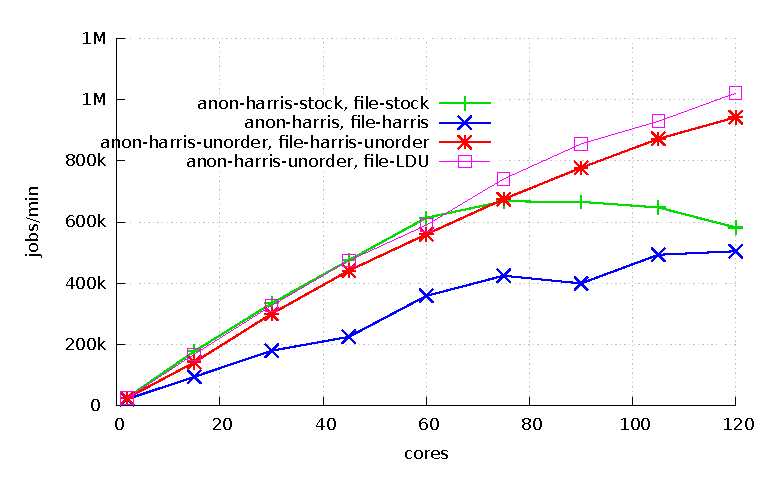
\includegraphics[scale=0.65]{graph/aim7.eps}
%  \end{center}
%  \caption{Scalability of AIM7 multiuser for different method.  The combination
%  \deferu with unordered harris list scale well;in contrast, up to 60 core, the
%  stock Linux scale linearly, then it  flattens out.}
%  \label{fig:aim7}
%\end{figure}

%Paragraph 1: 워크로드에 대한 설명
%AIM7 forks many processes, each of which concurrently runs. 
%We used AIM7-multiuser, which is one of workload in AIM7.
%The multiuser workload is composed of various workloads such as disk-file
%operations, process creation, virtual memory operations, pipe I/O, and
%arithmetic operation.
%To minimize IO bottlenecks, the workload was executed with tmpfs filesystems,
% each of which is 10 GB.
%To increase the number of users during our experiment and show the results at
% the peak user numbers, 
%we used the crossover.

%Paragraph 2: 실험 결과에 대한 설명
%The results for AIM7-multiuser are shown in Figure~\ref{fig:aim7}, and the
%results show the throughput of AIM7-multiuser with four different settings.
%Up to 60 core, the stock Linux scales linearly while serialized updates in
%Linux kernel become bottlenecks. 
%However, up to 120core, unordered harris list and our \deferu scale well
% because these workloads can run concurrently updates and can reduce the locking
%overheads due to reader-writer semaphores(\code{anon\_vma},
%\code{file}).
%The combination of \deferu with unordered harris list has best performance and
%scalability outperforming stock Linux by 1.7x and unordered harris list by
%1.1x.
%While the unordered harris list has 19\% idle time(see
%Table~\ref{tab:memuse}), stock Linux has 51\% idle time waiting to acquire
%both \code{anon\_vma's rwsem} and \code{file's i\_mmap\_rwsem}.
%We can notice that although \deferu has 23\% idle time, the throughput is
% higher than unordered harris list.
%In this benchmark, the ordered harris list has the lowest performance and
%scalability because their \code{CAS} fails frequently.

%\subsection{Exim}
% EXIM 실험 결과
%\begin{figure}[tb]
%  \begin{center}
%    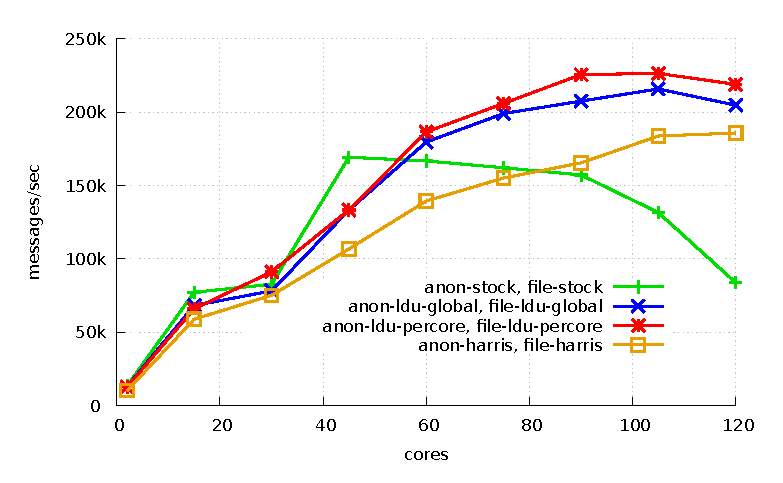
\includegraphics[scale=0.65]{graph/exim.eps}
%  \end{center}
%  \caption{Scalability of Exim. The stock Linux collapses after 60 core;in
%  contrast, both unordered harris list and our \deferu flatten out.}
%  \label{fig:exim}
%\end{figure}

%\begin{table}
%  \centering
%  \small
%  \begin{tabular}{l r r r } \toprule
%    AIM7 & user & sys & idle \\
%    \midrule
%    Stock(anon, file) & 2487 s & 1993 s & 4647 s(51\%)\\ 
%    H(anon, file) & 1123 s & 3631 s & 2186 s(31\%)\\
%    H-unorder(anon, flie) & 3630 s & 2511 s & 1466 s(19\%)\\
%    H-unorder(anon), L(file) & 3630 s & 1903 s & 1662 s(23\%)\\
%    \bottomrule
%  \end{tabular}
%  \begin{tabular}{l r r r } \toprule
%    EXIM & user & sys & idle \\
%    \midrule
%    Stock(anon, file) & 41 s & 499 s & 1260 s(70\%)\\ 
%    H(anon, file) & 47 s & 628 s & 1124 s(62\%)\\
%    H-unorder(anon, file) & 112 s & 1128 s & 559 s(31\%)\\
%    H-unorder(anon), L(file) & 87 s & 1055 s & 657 s(37\%)\\
%    \bottomrule
%  \end{tabular}
%  \begin{tabular}{l r r r } \toprule
%    lmbench & user & sys & idle \\
%    \midrule
%    Stock(anon, file) & 11 s & 208 s & 2158 s(91\%)\\ 
%    H(anon, file) & 11 s & 312 s & 367 s(53\%)\\
%    H-unorder(anon, file) & 11 s & 292 s & 315 s(51\%)\\
%    H-unorder(anon), L(file) & 12 s & 347 s & 349 s(49\%)\\
%    \bottomrule
%  \end{tabular}

%  \caption{Comparison of user, system and idle time at 120 cores.}
%  \label{tab:memuse}
%\end{table}


%Paragraph 1: 워크로드에 대한 설명
%To measure the performance of Exim, shown in Figure~\ref{fig:exim}, we
%used default value of MOSBENCH to use tmpfs for
%spool files, log files, and user mail files.
%Clients run on the same machine and each client sends to a different user to
%prevent contention on user mail file.
%The Exim was bottlenecked by per-directory locks protecting file creation in
%the spool directories and by forks performed on different
%cores~\cite{SilasBoydWickizer2010LinuxScales48}.
%Therefore, although we eliminate the fork problem, the Exim may suffer from
%contention on spool directories. 

%Paragraph 2:실험 결과에 대한 설명
%Results shown in Figure~\ref{fig:exim} show that Exim scales well for all
%methods up to 60 core but not for higher core counts.
%The stock Linux shows performance degradation for more than 60 core.
%Both unordered harris list
%and our \deferu do not suffer from performance loss 
%because they do not acquire the \code{anon\_vma}
%semaphore and \code{i\_mmap} semaphore in fork.
%\deferu performs better due to the fact that it uses both update-side
%absorbing and lock-less list, outperforming stock Linux by 1.6x and unordered
%harris list by 1.1x.
%Even though we applied scalable solution, Exim shows limitation on scalability
%improvement
%since the main bottleneck is per-directory lock contention on spool
%directories.
%The unordered harris list has 31\% idle time, whereas \deferu has 37\% idle
%time due to the their efficient concurrent updates.

%\subsection{lmbench}
%\begin{figure}[tb]
%  \begin{center}
%    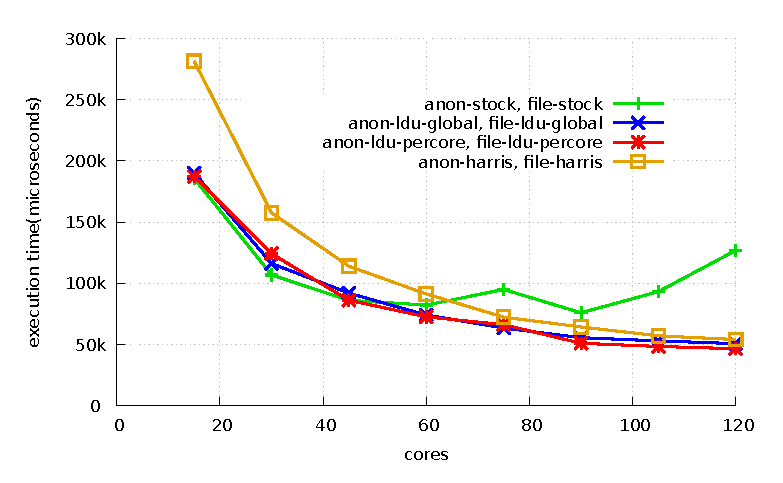
\includegraphics[scale=0.65]{graph/lmbench.eps}
%  \end{center}
%  \caption{Execution time of lmbench's fork micro benchmark. The fork micro
%  benchmark drops down for all methods up to 15 core but either flattens out or
%  goes up slightly after that. At 15 core, the stock Linux goes up;the others
%  flattens out}
%  \label{fig:MicroBench}
%\end{figure}

%Paragraph 1: %워크로드에 대한 설명
%lmbench has various workloads including process creation workload(fork,
%exec, sh -c, exit).
%This workload is used to measure the basic process primitives such as creating
%a new process, running a different program, and context switching. 
%We configured process create workload to enable the parallelism option which
%specifies the number of benchmark processes to run in
%parallel~\cite{mcvoy1996lmbench}; we used 100 processes.

%Paragraph 2: 실험 결과에 대한 설명
%The results for lmbench are shown in Figure~\ref{fig:MicroBench}, 
%and the results show the execution times of the fork microbenchmark in lmbench
%with four different methods.
%The fork micro benchmark drops down for all methods up to 15 core but either
%flattens out or goes up slightly after that.
%Three methods outperform stock Linux by 2.2x at 120 cores;however, before 30
%core, two harris list have lower performance due to their execution overheads.
%At 15 core, the stock Linux goes up because of the NUMA effect that accesses
%the remote memory.
%On the other hand, the others including the ordered harris list flattens out
%and then they remain constant.
%While stock Linux has 90\% idle time, other methods have approximately 50\%
%idle time since stock Linux waits to acquire reverse mapping locks such as
%\code{anon\_vma's rwsem} and \code{mapping's i\_mmap\_rwsem}.

\section{Discussion}

%$$$$$$$$$$$$$$$$$$$$$$$$$$$$$$$$$$$$$$$$$$$$$$$$$$$$$$$$$$$$$$$$$$$$$$$$$$$$$$$$
%Paragraph 1: 더 범용적이게 만들어야 한다.
%$$$$$$$$$$$$$$$$$$$$$$$$$$$$$$$$$$$$$$$$$$$$$$$$$$$$$$$$$$$$$$$$$$$$$$$$$$$$$$$$
\ifkor
우리는 리눅스 커널과 같이 update operation이 insert-insert또는 remove-remove와 같이 같은 operation에
대해서 발생하지 않는 data structure의 경우에 대해서만 사용 가능하도록 LDU를 구현하였다.
이러한 방법은 굉장히 practical한 방법으로 리눅스와 freeBSD와 같은 커널에는 적용 할 수 있으나 
보다 연구 중심적인 data structure인 CSDS 알고리즘과 비교 실험하는데는 무리가 있다. 
따라서 LDU 또는 Oplog와 같이 log-based 방법을 보다 연구 중심적인 data structure와 비교 실험이
가능하도록 보다 일반화할 필요가 있다. 
\else

\fi

%$$$$$$$$$$$$$$$$$$$$$$$$$$$$$$$$$$$$$$$$$$$$$$$$$$$$$$$$$$$$$$$$$$$$$$$$$$$$$$$$
%$$$$$$$$$$$$$$$$$$$$$$$$$$$$$$$$$$$$$$$$$$$$$$$$$$$$$$$$$$$$$$$$$$$$$$$$$$$$$$$$
%Reference Sentence 1
%$$$$$$$$$$$$$$$$$$$$$$$$$$$$$$$$$$$$$$$$$$$$$$$$$$$$$$$$$$$$$$$$$$$$$$$$$$$$$$$$





%$$$$$$$$$$$$$$$$$$$$$$$$$$$$$$$$$$$$$$$$$$$$$$$$$$$$$$$$$$$$$$$$$$$$$$$$$$$$$$$$
%Reference Sentence 2:LDU paper
%$$$$$$$$$$$$$$$$$$$$$$$$$$$$$$$$$$$$$$$$$$$$$$$$$$$$$$$$$$$$$$$$$$$$$$$$$$$$$$$$


\section{Related work} \label{sec:RelatedWork}
%$$$$$$$$$$$$$$$$$$$$$$$$$$$$$$$$$$$$$$$$$$$$$$$$$$$$$$$$$$$$$$$$$$$$$$$$$$$$$$$$
%Paragraph 1:Linux Scalability의 연구에 대한 설명
%$$$$$$$$$$$$$$$$$$$$$$$$$$$$$$$$$$$$$$$$$$$$$$$$$$$$$$$$$$$$$$$$$$$$$$$$$$$$$$$$
\ifkor
\noindent
\textbf{Operating system scalability.}
~\cite{Clements15SCR}In order to improve Linux scalability, researchers have
been optimized memory management in Linux by finding and fixing scalability
bottlenecks~\cite{BoydWickizer2008Corey}~\cite{BoydWickizer2012OLS}.
Shared address spaces in multithreaded applications 
easily become scalability bottlenecks since kernel operations 
including \code{mmap} and \code{munmap} system calls and \code{page faults}
 handling require per-process locks for synchronization.
Multithreaded application, for example, can become bottleneck by kernel
operations on their shared address space, whose operations are the \code{mmap}
and \code{munmap} system calls and \code{page faults}.
These operations are synchronized by a single per-process lock.
BonsaiVM~\cite{AustinTClements2012RCUBalancedTrees} solved this address space
problem by using the RCU;
RadixVM~\cite{Clements2013RadixVM} created a new VM using refcache and radix
tree, which enable \code{munmap}, \code{mmap}, and \code{page fault} on
non-overlapping memory regions to scale perfectly.
Alternatively, to avoid contention caused by shared address space locking,
system programmers change their multithreaded applications to use
processes~\cite{SilasBoydWickizer2010LinuxScales48}.
\else

\fi


%$$$$$$$$$$$$$$$$$$$$$$$$$$$$$$$$$$$$$$$$$$$$$$$$$$$$$$$$$$$$$$$$$$$$$$$$$$$$$$$$
%Paragraph 2:Concurrent updates에 대한 연구
%$$$$$$$$$$$$$$$$$$$$$$$$$$$$$$$$$$$$$$$$$$$$$$$$$$$$$$$$$$$$$$$$$$$$$$$$$$$$$$$$
\ifkor
\noindent
\textbf{Scalabe data structure.}
~\cite{Dodds2015SCT}Though sufficient level of performance scalability has been
achieved for reader intensive operations through RCU and Hazard pointer, 
solutions to scalability for update-heavy operations has not been satisfiable.
A recent paper by Arbel and Attiya~\cite{Arbel2014ConcurrentRCU} shows a new
design of concurrent search tree called the Citrus tree. The Citrus tree
combines RCU and fine-grained locks, and it supports concurrent write
operations that traverse the search tree by using RCU concurrently.
When increasing the update rate, Citrus tree still suffers from bottlenecks.
RLU~\cite{Matveev2015RLU} presents a new synchronization mechanism that allows
unsynchronized sequences of reads to execute concurrently with updates.
In high update rate, Oplog can achieve substantially multi-core scaling for
update-heavy data structures.
Our work focus on update-heavy data structures and uses non-blocking method to
 store the operation log instead of per-core processing.
\else

\fi



%$$$$$$$$$$$$$$$$$$$$$$$$$$$$$$$$$$$$$$$$$$$$$$$$$$$$$$$$$$$$$$$$$$$$$$$$$$$$$$$$
%Paragraph 3: Scalable Data Structure and Lock에 대한 연구
%$$$$$$$$$$$$$$$$$$$$$$$$$$$$$$$$$$$$$$$$$$$$$$$$$$$$$$$$$$$$$$$$$$$$$$$$$$$$$$$$
\ifkor
\noindent
\textbf{Scalable lock.}
~\cite{Wang2016BeMyGuest}~\cite{Bueso2015STP}~\cite{Bueso2014MCS}One method for
the concurrent update is using the non-blocking algorithms~\cite{Harris2001Lockfree}~\cite{Fomitchev2004Lockfree}~\cite{Timnat2012},
 which are based on CAS.


MCS~\cite{MellorCrummey91}, a scalable exclusive lock, is used in the Linux
kernel~\cite{MCSLocksKernel}.
to avoid unfairness at high contention levels, so this scalable exclusive
lock can be used for fine grained locking in Linux. 
However, in MCS, since only one thread may hold the lock at a time, it can
cause low scalability in case of long critical regions.
Reader-writer lock~\cite{Courtois71} allows either number of readers to execute
concurrently or single writer to execute.
Thus, readers-writer locks allow better scalability in case of read-mostly 
objects.

In read-mostly data structures, RCU~\cite{McKenney98} can be quite useful
since it allows read operations to proceed without read locks, and delays
freeing of data structures to avoid races. One drawback is that as the update
rate increases, their performance and scalability decrease due to a single
writer and their synchronization function.
Consequently, 
scalable exclusive lock, reader-writer lock
and RCU require serialization for updates and thus show significant limitation
 on scalability. 
\else

\fi




%$$$$$$$$$$$$$$$$$$$$$$$$$$$$$$$$$$$$$$$$$$$$$$$$$$$$$$$$$$$$$$$$$$$$$$$$$$$$$$$$
%$$$$$$$$$$$$$$$$$$$$$$$$$$$$$$$$$$$$$$$$$$$$$$$$$$$$$$$$$$$$$$$$$$$$$$$$$$$$$$$$
%Reference Sentence 1
%$$$$$$$$$$$$$$$$$$$$$$$$$$$$$$$$$$$$$$$$$$$$$$$$$$$$$$$$$$$$$$$$$$$$$$$$$$$$$$$$




%$$$$$$$$$$$$$$$$$$$$$$$$$$$$$$$$$$$$$$$$$$$$$$$$$$$$$$$$$$$$$$$$$$$$$$$$$$$$$$$$
%Reference Sentence 2:LDU paper
%$$$$$$$$$$$$$$$$$$$$$$$$$$$$$$$$$$$$$$$$$$$$$$$$$$$$$$$$$$$$$$$$$$$$$$$$$$$$$$$$

%Paragraph 1:Linux Scalability의 연구에 대한 설명
%In order to improve Linux scalability, researchers have been optimized memory
%management in Linux by finding and fixing scalability bottlenecks.

%Shared address spaces in multithreaded applications 
%easily become scalability bottlenecks since kernel operations 
%including \code{mmap} and \code{munmap} system calls and \code{page faults}
% handling require per-process locks for synchronization.
%Multithreaded application, for example, can become bottleneck by kernel
%operations on their shared address space, whose operations are the \code{mmap}
%and \code{munmap} system calls and \code{page faults}.
%These operations are synchronized by a single per-process lock.
%BonsaiVM~\cite{AustinTClements2012RCUBalancedTrees} solved this address space
%problem by using the RCU;
%RadixVM~\cite{Clements2013RadixVM} created a new VM using refcache and radix
%tree, which enable \code{munmap}, \code{mmap}, and \code{page fault} on
%non-overlapping memory regions to scale perfectly.
%Alternatively, to avoid contention caused by shared address space locking,
%system programmers change their multithreaded applications to use
%processes~\cite{SilasBoydWickizer2010LinuxScales48}.
 
%Paragraph 2:Fork Scalability에 대한 설명
%Multi-processing environment 
%suffers from scalability bottlenecks due to the well-known fork
%scalability problem~\cite{Andi2011adding}~\cite{Tim2013adding}.
%When Linux spawns child process, the Linux substantially performs locks because
%of protecting the reverse mapping data structure naturally causing
%bottlenecks.
%Oplog~\cite{SilasBoydWickizerPth}, which is an important basis of our approach,
%solves this problem using time-stamp log and
%per-core processing.


%\subsection{Locking}
%Paragraph 1: Locks에 대한 설명
%MCS~\cite{MellorCrummey91}, a scalable exclusive lock, is used in the Linux
%kernel~\cite{MCSLocksKernel}.
%to avoid unfairness at high contention levels, so this scalable exclusive
%lock can be used for fine grained locking in Linux. 
%However, in MCS, since only one thread may hold the lock at a time, it can
%cause low scalability in case of long critical regions.
%Reader-writer lock~\cite{Courtois71} allows either number of readers to execute
%concurrently or single writer to execute.
%Thus, readers-writer locks allow better scalability in case of read-mostly 
%objects.

%In read-mostly data structures, RCU~\cite{McKenney98} can be quite useful
%since it allows read operations to proceed without read locks, and delays
%freeing of data structures to avoid races. One drawback is that as the update
%rate increases, their performance and scalability decrease due to a single
%writer and their synchronization function.
%Consequently, 
%scalable exclusive lock, reader-writer lock
%and RCU require serialization for updates and thus show significant limitation
% on scalability. 

%\subsection{Non-Blocking algorithm}

%Paragraph 1: Lock-free 방법 설명
%One method for the concurrent update is using the non-blocking
%algorithms~\cite{Harris2001Lockfree}~\cite{Fomitchev2004Lockfree}~\cite{Timnat2012},
% which are based on CAS.
%In non-blocking algorithms, each core tries to read the values of shared
%data structures from its local location, but has possibility of reading 
%obsolete values.
%CAS is performed at the time of reading values that are not the current values
%and CAS fails and requires retrials sometimes when the values have been
% overwritten.
%These algorithms execute optimistically as though they read the value at
%location in their data structure;they may obtain stale data at the time.
%When they observed against the current value, they execute a CAS to compare the
%against value.
%The CAS fails when the value has been overridden, and they must be
%retried later on.
%Consequently, both repeated CAS operation and their iteration loop caused by
%CAS fails cause bottlenecks due to inter-core communication
% overheads~\cite{SilasBoydWickizerPth}.
%Moreover, none of the non-blocking algorithms implements an iterator, whose
%data structure just consists of the insert, delete and contains
%operations~\cite{petrank2013lock}.
%The Linux, however, commonly uses the iteration to read, so when applying
%non-blocking algorithms to the Linux, they may meet this iteration problem.
%Petrank~\cite{petrank2013lock} solved this problem by using a consistent
%snapshot of the data structure; this method, however, may require a lot of
%effort to apply its sophisticated algorithms to Linux.
%For evaluation purposes, we implemented Harris linked
%list~\cite{Harris2001Lockfree} to Linux, and we sometimes have failure where
%reading the pointer that had been deleted by updater concurrently result of the
%problem of the iteration.

%Paragraph 2: Linux llist 설명
%Linux kernel uses lock-less list("lock-less NULL terminated single
%list") that are widely used in the Linux kernel to improve scalability.
%In order to delete operation for multiple consumer, the existing
%algorithms traverse the list from beginning or their optimized point.
%On the other hand, lock-less list inserts node at the first of the list, so
% when the CAS operation fails, they will minimally traverse from the head
% node.
%Although lock-less list uses a non blocking method, they retries minimally
%and thus they can significantly reduce inter-core communication bottleneck and
% the repeated loop bottleneck.
%Our proposed method uses this feature in case of inserting the operation log.

%\subsection{Concurrent Update}
%Paragraph 1: Update Rate
%Though sufficient level of performance scalability has been achieved for 
%reader intensive operations through RCU and Hazard pointer, 
%solutions to scalability for update-heavy operations has not been satisfiable.
%A recent paper by Arbel and Attiya~\cite{Arbel2014ConcurrentRCU} shows a new
%design of concurrent search tree called the Citrus tree. The Citrus tree
%combines RCU and fine-grained locks, and it supports concurrent write
%operations that traverse the search tree by using RCU concurrently.
%When increasing the update rate, Citrus tree still suffers from bottlenecks.
%RLU~\cite{Matveev2015RLU} presents a new synchronization mechanism that allows
%unsynchronized sequences of reads to execute concurrently with updates.
%In high update rate, Oplog can achieve substantially multi-core scaling for
%update-heavy data structures.
%Our work focus on update-heavy data structures and uses non-blocking method to
% store the operation log instead of per-core processing.

\section{Conclusion}


\section{Acknowledgments}



%$$$$$$$$$$$$$$$$$$$$$$$$$$$$$$$$$$$$$$$$$$$$$$$$$$$$$$$$$$$$$$$$$$$$$$$$$$$$$$$$
%$$$$$$$$$$$$$$$$$$$$$$$$$$$$$$$$$$$$$$$$$$$$$$$$$$$$$$$$$$$$$$$$$$$$$$$$$$$$$$$$
%Reference Sentence 1
%$$$$$$$$$$$$$$$$$$$$$$$$$$$$$$$$$$$$$$$$$$$$$$$$$$$$$$$$$$$$$$$$$$$$$$$$$$$$$$$$


%$$$$$$$$$$$$$$$$$$$$$$$$$$$$$$$$$$$$$$$$$$$$$$$$$$$$$$$$$$$$$$$$$$$$$$$$$$$$$$$$
%$$$$$$$$$$$$$$$$$$$$$$$$$$$$$$$$$$$$$$$$$$$$$$$$$$$$$$$$$$$$$$$$$$$$$$$$$$$$$$$$
%Reference Sentence 2:LDU paper
%$$$$$$$$$$$$$$$$$$$$$$$$$$$$$$$$$$$$$$$$$$$$$$$$$$$$$$$$$$$$$$$$$$$$$$$$$$$$$$$$

%We propose a concurrent update algorithm, \deferu, for update-heavy data
%structures scalable for many-core systems.
%To achieve the scalability during process spawning, 
%we applied deferred log processing with global log queue and 
%update-side absorbing to Linux reverse mapping.
%Evaluation results using the AIM7, Exim and lmbench reveal that \deferu shows
%better performance up to 2.2 times compared to existing solutions.
%\deferu is implemented on to Linux kernel 3.19 and available as open-source
% from \url{https://github.com/KMU-embedded/scalablelinux}.

%\section{Acknowledgments}
%This work was supported by Institute for Information \& communications
% Technology Promotion (IITP) grant funded by the Korea government (MSIP) (14-824-09-
%011, “Research Project on High Performance and Scalable Manycore Operating
% System”)



\bibliographystyle{plain}
\bibliography{ref}

\ifkor
\end{CJK}
\fi

% \section{Introduction}
% no \IEEEPARstart
% This demo file is intended to serve as a ``starter file''
% % for IEEE conference papers produced under \LaTeX\ using
% IEEEtran.cls version 1.7 and later.

% All manuscripts must be in English. These guidelines include complete
% descriptions of the fonts, spacing, and related information for producing your proceedings manuscripts. Please follow them and if you have any questions, direct them to the production editor in charge of your proceedings at Conference Publishing Services (CPS): Phone +1 (714) 821-8380 or Fax +1 (714) 761-1784.
% You must have at least 2 lines in the paragraph with the drop letter
% (should never be an issue)

% \subsection{Subsection Heading Here}
% Subsection text here.


% \subsubsection{Subsubsection Heading Here}
% Subsubsection text here.

% \section{Type style and Fonts}
% Wherever Times is specified, Times Roman or Times New Roman may be used. If
% neither is available on your system, please use the font closest in appearance to Times. Avoid using bit-mapped fonts if possible. True-Type 1 or Open Type fonts are preferred. Please embed symbol fonts, as well, for math, etc.


% An example of a floating figure using the graphicx package.
% Note that \label must occur AFTER (or within) \caption.
% For figures, \caption should occur after the \includegraphics.
% Note that IEEEtran v1.7 and later has special internal code that
% is designed to preserve the operation of \label within \caption
% even when the captionsoff option is in effect. However, because
% of issues like this, it may be the safest practice to put all your
% \label just after \caption rather than within \caption{}.
%
% Reminder: the "draftcls" or "draftclsnofoot", not "draft", class
% option should be used if it is desired that the figures are to be
% displayed while in draft mode.
%
%\begin{figure}[!t]
%\centering
%\includegraphics[width=2.5in]{myfigure}
% where an .eps filename suffix will be assumed under latex, 
% and a .pdf suffix will be assumed for pdflatex; or what has been declared
% via \DeclareGraphicsExtensions.
%\caption{Simulation Results}
%\label{fig_sim}
%\end{figure}

% Note that IEEE typically puts floats only at the top, even when this
% results in a large percentage of a column being occupied by floats.


% An example of a double column floating figure using two subfigures.
% (The subfig.sty package must be loaded for this to work.)
% The subfigure \label commands are set within each subfloat command, the
% \label for the overall figure must come after \caption.
% \hfil must be used as a separator to get equal spacing.
% The subfigure.sty package works much the same way, except \subfigure is
% used instead of \subfloat.
%
%\begin{figure*}[!t]
%\centerline{\subfloat[Case I]\includegraphics[width=2.5in]{subfigcase1}%
%\label{fig_first_case}}
%\hfil
%\subfloat[Case II]{\includegraphics[width=2.5in]{subfigcase2}%
%\label{fig_second_case}}}
%\caption{Simulation results}
%\label{fig_sim}
%\end{figure*}
%
% Note that often IEEE papers with subfigures do not employ subfigure
% captions (using the optional argument to \subfloat), but instead will
% reference/describe all of them (a), (b), etc., within the main caption.


% An example of a floating table. Note that, for IEEE style tables, the 
% \caption command should come BEFORE the table. Table text will default to
% \footnotesize as IEEE normally uses this smaller font for tables.
% The \label must come after \caption as always.
%
%\begin{table}[!t]
%% increase table row spacing, adjust to taste
%\renewcommand{\arraystretch}{1.3}
% if using array.sty, it might be a good idea to tweak the value of
% \extrarowheight as needed to properly center the text within the cells
%\caption{An Example of a Table}
%\label{table_example}
%\centering
%% Some packages, such as MDW tools, offer better commands for making tables
%% than the plain LaTeX2e tabular which is used here.
%\begin{tabular}{|c||c|}
%\hline
%One & Two\\
%\hline
%Three & Four\\
%\hline
%\end{tabular}
%\end{table}


% Note that IEEE does not put floats in the very first column - or typically
% anywhere on the first page for that matter. Also, in-text middle ("here")
% positioning is not used. Most IEEE journals/conferences use top floats
% exclusively. Note that, LaTeX2e, unlike IEEE journals/conferences, places
% footnotes above bottom floats. This can be corrected via the \fnbelowfloat
% command of the stfloats package.



% \section{Conclusion}
% The conclusion goes here. this is more of the conclusion

% conference papers do not normally have an appendix


% use section* for acknowledgement
% \section*{Acknowledgment}


% The authors would like to thank...
% more thanks here


% trigger a \newpage just before the given reference
% number - used to balance the columns on the last page
% adjust value as needed - may need to be readjusted if
% the document is modified later
%\IEEEtriggeratref{8}
% The "triggered" command can be changed if desired:
%\IEEEtriggercmd{\enlargethispage{-5in}}

% references section

% can use a bibliography generated by BibTeX as a .bbl file
% BibTeX documentation can be easily obtained at:
% http://www.ctan.org/tex-archive/biblio/bibtex/contrib/doc/
% The IEEEtran BibTeX style support page is at:
% http://www.michaelshell.org/tex/ieeetran/bibtex/
%\bibliographystyle{IEEEtran}
% argument is your BibTeX string definitions and bibliography database(s)
%\bibliography{IEEEabrv,../bib/paper}
%
% <OR> manually copy in the resultant .bbl file
% set second argument of \begin to the number of references
% (used to reserve space for the reference number labels box)
% \begin{thebibliography}{1}

% \bibitem{IEEEhowto:kopka}
% H.~Kopka and P.~W. Daly, \emph{A Guide to \LaTeX}, 3rd~ed.\hskip 1em plus
%   0.5em minus 0.4em\relax Harlow, England: Addison-Wesley, 1999.
% \end{thebibliography}




% that's all folks
\end{document}


